
\newif\ifcrossling\crosslingtrue
\newif\ifitmtree\itmtreetrue
\newif\iflong\longtrue
\newif\ifevaluation\evaluationfalse
\newif\ifconjugacy\conjugacytrue
\newif\ifnonpar\nonparfalse
\newif\ifling\lingfalse
\newif\ifhighlevel\highlevelfalse
\newif\iftmreview\tmreviewfalse
\newif\ifevocation\evocationfalse
\newif\ifsupershortmlslda\supershortmlsldatrue

\documentclass[compress]{beamer}

%\usepackage{beamerthemesplit}
\usepackage{xmpmulti}

\definecolor{green}{rgb}{0,.3,0}

\usepackage{graphicx,float,wrapfig, bbm}
\usepackage{amsfonts, bbold, comment}
\usepackage{mdwlist}
\usepackage{listings}
\usepackage{environ}
\usepackage{subfigure}
\usepackage{rotating}
\usepackage{algorithmic}
\usepackage{algorithm}
\usepackage{overpic}

\usepackage{multirow}

\usetheme{Rochester}
%\useoutertheme{infolines}
%\usetheme{Boadilla}
%\usetheme{Singapore}
\usecolortheme{umd}
\title{Topic Models}
\author{Jordan Boyd-Graber}
\date{1. April 2014}

\newcommand{\explain}[2]{\underbrace{#2}_{\mbox{\footnotesize{#1}}}}
\newcommand{\dir}[1]{\mbox{Dir}(#1)}
\newcommand{\mult}[1]{\mbox{Mult}( #1)}
\newcommand{\Beta}[1]{\mbox{Beta}( #1)}
\newcommand{\G}[1]{\Gamma \left( \textstyle #1 \right)}
\newcommand{\LG}[1]{\log \Gamma \left( \textstyle #1 \right)}
\newcommand{\WN}[0]{\textsc{WordNet}}
\newcommand{\itmspace}[0]{\hspace{2cm}}
\newcommand{\abr}[1]{\textsc{#1}}
\newcommand{\lda}[0]{\abr{lda}}
\newcommand{\slda}[0]{\abr{slda}}

\newcommand{\digam}[1]{\Psi \left( \textstyle #1 \right) }
\newcommand{\ddigam}[1]{\Psi' \left( \textstyle #1 \right) }
\newcommand{\e}[2]{\mathbb{E}_{#1}\left[ #2 \right] }
\newcommand{\ind}[1]{\mathbb{I}\left[ #1 \right] }
\newcommand{\ex}[1]{\mbox{exp}\left\{ #1\right\} }
\newcommand{\D}[2]{\frac{\partial #1}{\partial #2}}
\newcommand{\elbo}{\mathcal{L}}


\newcommand{\citename}[1]{\emph{#1} }
\newcommand{\bm}[1]{\mbox{\boldmath$#1$}}
\newcommand{\Dir}{\mathrm{Dir}}
\newcommand{\Mult}{\mathrm{Mult}}
\newcommand{\g}[1]{\Gamma \left( #1 \right)}
\newcommand{\paragraph}[1]{ \vskip 1cm {\bf \large #1}}

\NewEnviron{smalign}{
\vspace{-.6cm}
\begin{small}
\begin{align}
  \BODY
\end{align}
\end{small}
\vspace{-.6cm}
}


\providecommand{\graphscale}{0.6}

\newcommand{\danquote}[1]{

\begin{flushright}
\begin{overpic}[width=5.5cm,tics=10]{general_figures/speech_bubble}
	\put(10,30) { \parbox{4cm}{#1 }}
\end{overpic}

\includegraphics[width=1.5cm]{general_figures/milkman_dan}
\end{flushright}
}


\AtBeginSection[] % "Beamer, do the following at the start of every section"
{ \begin{frame}

\frametitle{Outline} % make a frame titled "Outline"
\tableofcontents[currentsection] % show TOC and highlight current section
\end{frame} }

\lstset{language=Python,basicstyle=\tiny}

\DeclareMathSymbol{\R}{\mathbin}{AMSb}{"52}

%\setbeamertemplate{footline}{\hspace*{.5cm}\scriptsize{\insertauthor

\begin{document}

\frame{\titlepage

\centering

\includegraphics[width=0.2\linewidth]{general_figures/umd_logo} \\
}

\section{Topic Model Introduction}



\providecommand{\graphscale}{0.6}


\newcommand{\dirfunc}[3]{ \frac{ \prod_{#1}^{#2} \g{ #3 } } { \g{ \sum_{#1}^{#2} #3 }}}
\newcommand{\dirnum}[4]{ \frac{\g{ #3 }}{#4} \prod_{#1}^{#2} }
\newcommand{\dirden}[3]{ \g{ \sum_{#1}^{#2} #3 } }



\begin{frame}

	\frametitle{Why topic models?}

	\begin{columns}

	\column{.3\linewidth}

	
\includegraphics[width=1\linewidth]{topic_models/newspapers}

	\column{.55\linewidth}

	\begin{itemize}
		\item Suppose you have a huge number of documents
		\item Want to know what's going on
		\item Can't read them all (e.g. every New York Times article from the 90's)
		\item Topic models offer a way to get a corpus-level view of major themes
		\pause
		\item Unsupervised
	\end{itemize}


	\end{columns}

\end{frame}

\frame{
\begin{center}
\frametitle{Conceptual Approach}
From an \textbf<1>{input corpus} and number of topics \textbf<1>{$K$} $\rightarrow$ \textbf<2>{words to topics} \\
\only<1>{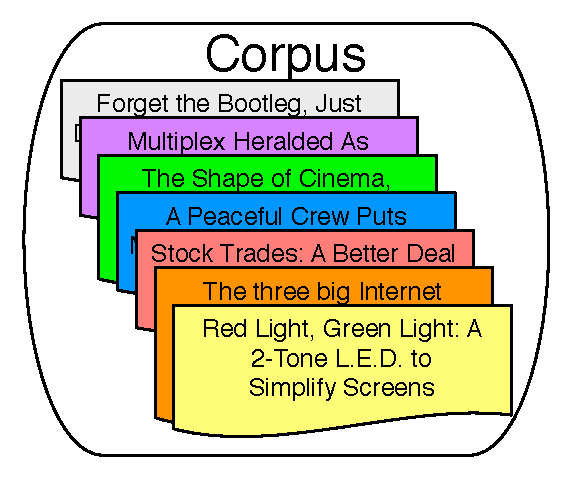
\includegraphics[width=0.6\linewidth]{reading_tea_leaves/figures/heldout_0} }
\only<2>{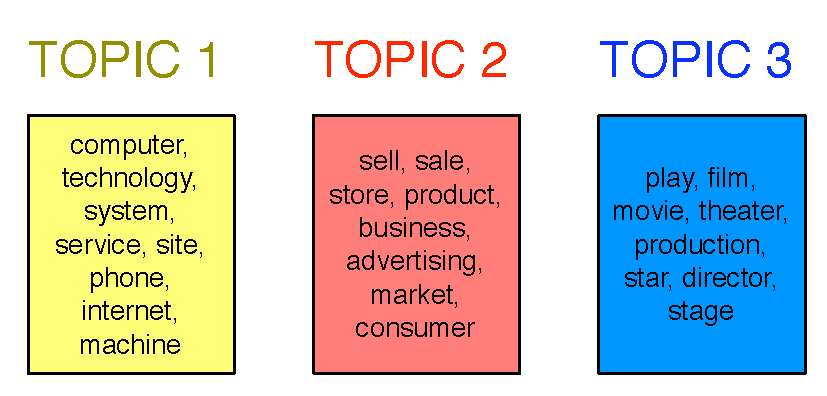
\includegraphics[width=0.9\linewidth]{reading_tea_leaves/figures/nyt_topics_wide}}
\end{center}
}

\frame{\frametitle{Conceptual Approach}

\begin{itemize}
\item For each document, what topics are expressed by that document?

\begin{center}
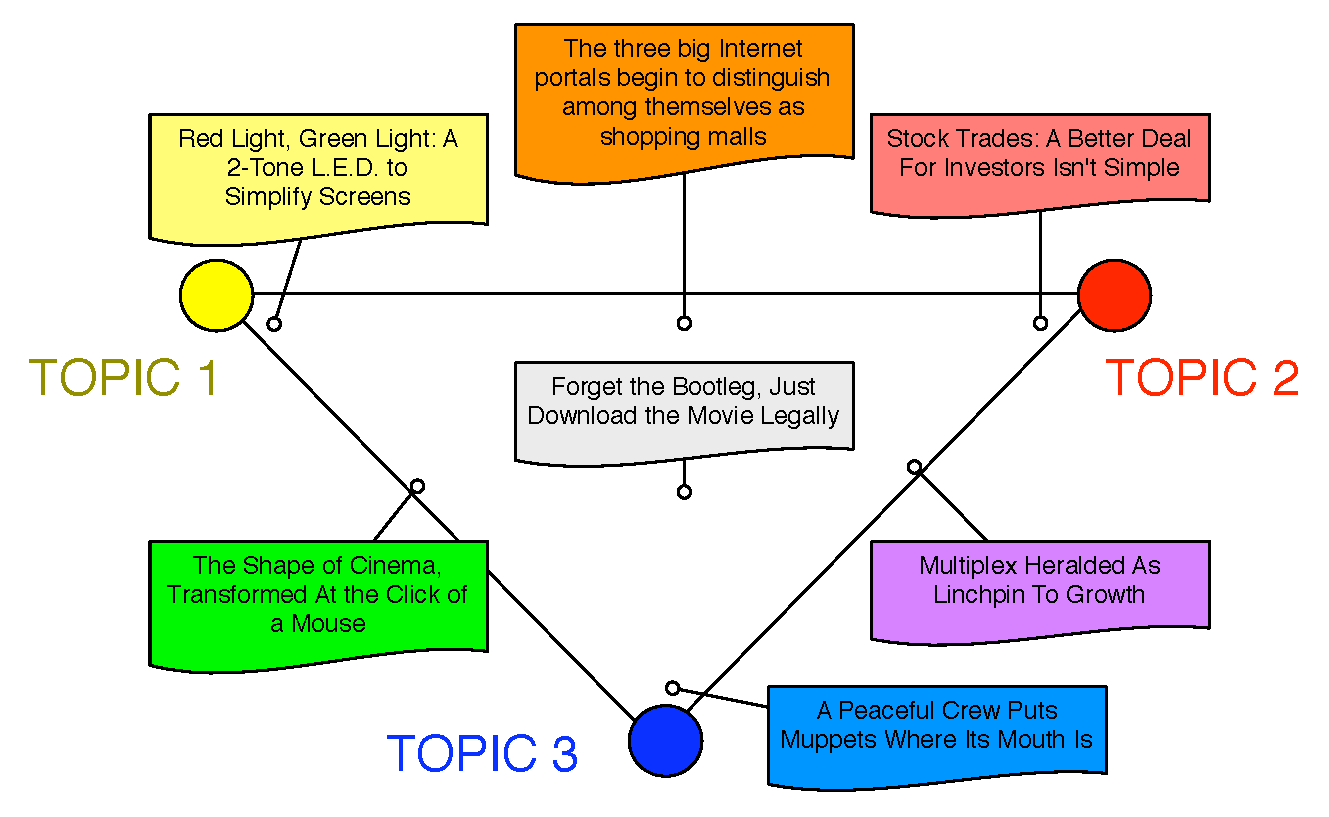
\includegraphics[width=0.9\linewidth]{topic_models/nyt_documents}
\end{center}

\end{itemize}
}


\begin{frame}

\frametitle{Topics from \emph{Science}}

\begin{center}
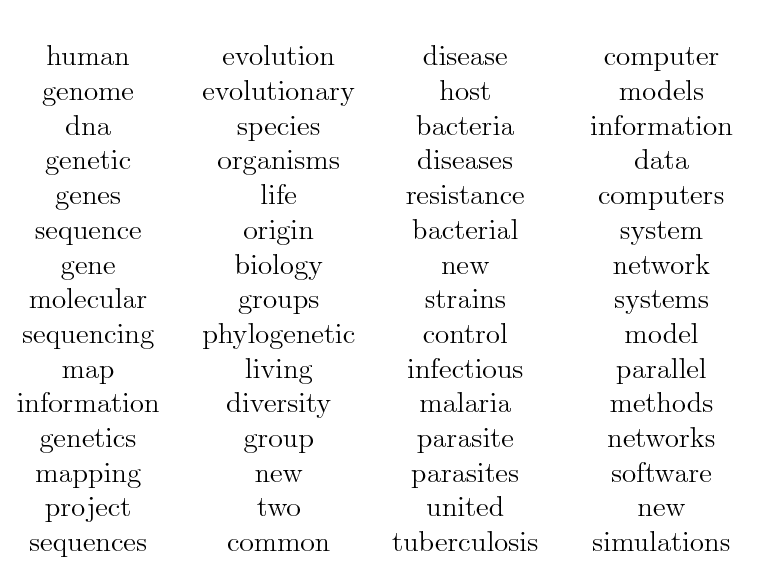
\includegraphics[width=0.8\linewidth]{topic_models/example_topics}
\end{center}

\end{frame}


\begin{frame}

\frametitle{Why should you care?}

\begin{itemize}
\item Neat way to explore / understand corpus collections
\begin{itemize}
	\item E-discovery
	\item Social media
	\item Scientific data
\end{itemize}
\item NLP Applications
\begin{itemize}
   \item POS Tagging~\cite{toutanova-08}
   \item Word Sense Disambiguation~\cite{boyd-graber-07}
   \item Word Sense Induction~\cite{brody-09}
   \item Discourse Segmentation~\cite{purver-06}
\end{itemize}
\item Psychology~\cite{griffiths-07}: word meaning, polysemy
\item Inference is (relatively) simple
\end{itemize}


\end{frame}


\section{Definition and Derivation}



\frame
{
  \frametitle{Matrix Factorization Approach}

\begin{center}
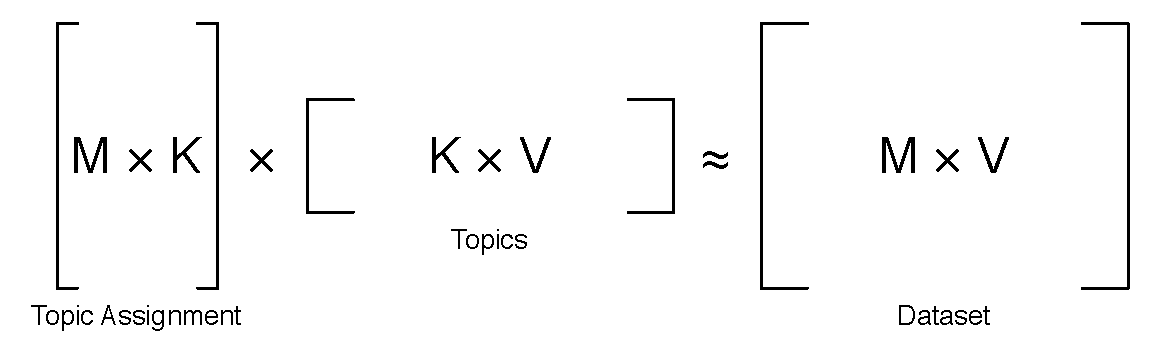
\includegraphics[width=0.9\linewidth]{topic_models/factorization.pdf}
\end{center}

\begin{columns}
\column{.5\textwidth}
\begin{block}{}
	\begin{itemize}
		\item[K] Number of topics
		\item[M] Number of documents
		\item[V] Size of vocabulary
	\end{itemize}
\end{block}
\column{.5\textwidth}
\pause
\begin{itemize}
\item If you use singular value decomposition (SVD), this technique is called latent semantic analysis.
\item Popular in information retrieval.
\end{itemize}
\end{columns}

}

\begin{frame}

\frametitle{Alternative: Generative Model}

\begin{itemize}
  \item How your data came to be
  \item Sequence of Probabilistic Steps
  \item Posterior Inference
\end{itemize}

\end{frame}

\begin{frame}
	\frametitle{Multinomial Distribution}

	\begin{itemize}
		\item Distribution over discrete outcomes
		\item Represented by non-negative vector that sums to one
		\item Picture representation
	\begin{center}
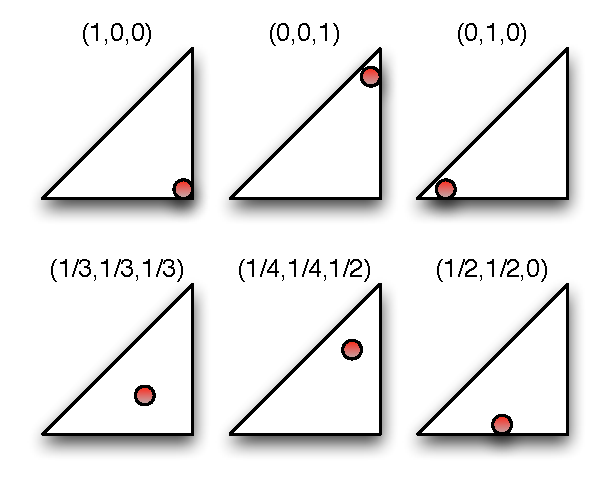
\includegraphics[width=0.4\linewidth]{topic_models/multinomial}
	\end{center}
		\pause
		\item Come from a Dirichlet distribution

	\end{itemize}

        \pause

        \vspace{-5cm}

        \begin{block}{Look familiar?}
          \centering
          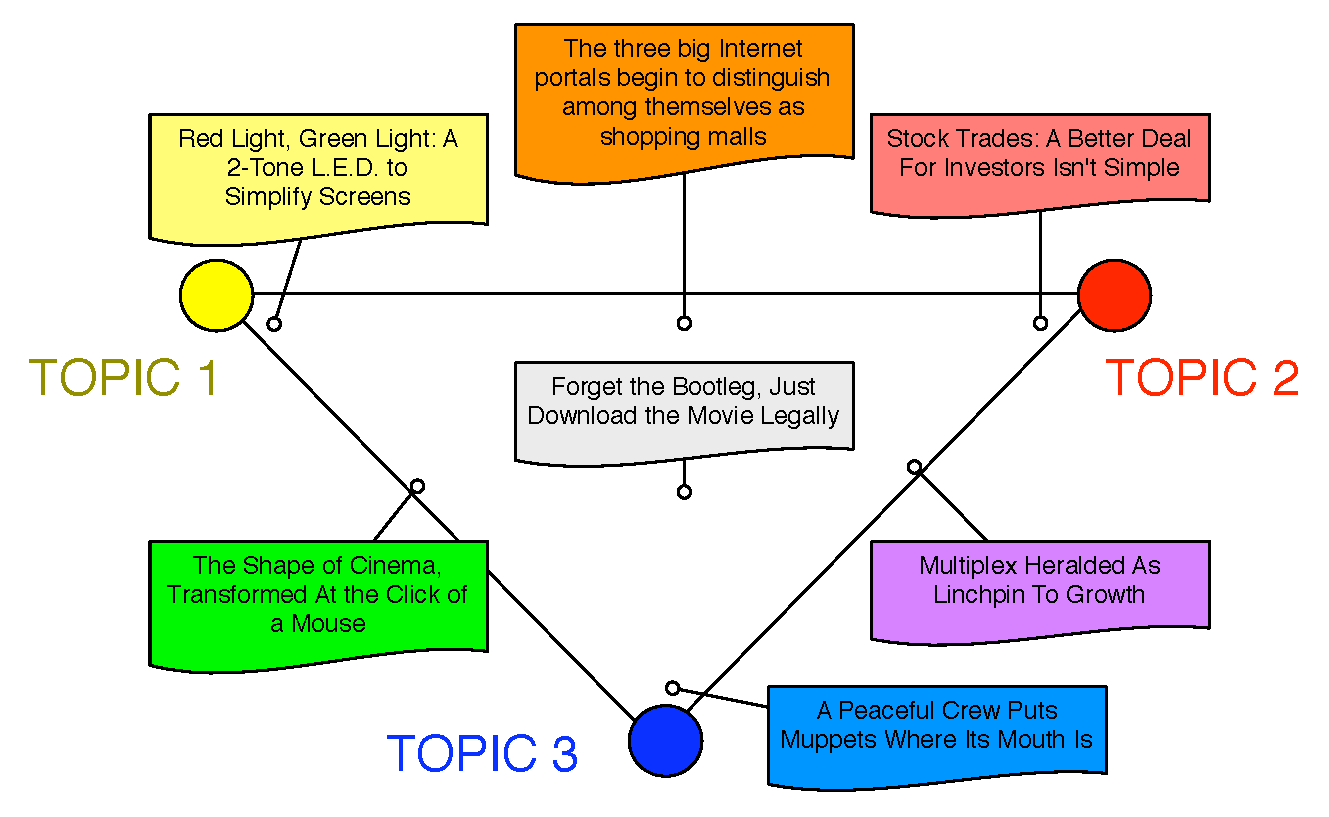
\includegraphics[width=0.7\linewidth]{topic_models/nyt_documents}
        \end{block}

\end{frame}

\begin{frame}

\frametitle{Dirichlet Distribution}

\begin{center}
\begin{equation}
  p(\theta | \vec{\alpha}) = \frac{ \Gamma \left( \sum_k \alpha_k \right)}{\prod_k \Gamma(\alpha_k)} \prod_k \theta_k^{\alpha_k = 1}
\end{equation}
\bigskip

\only<2>{
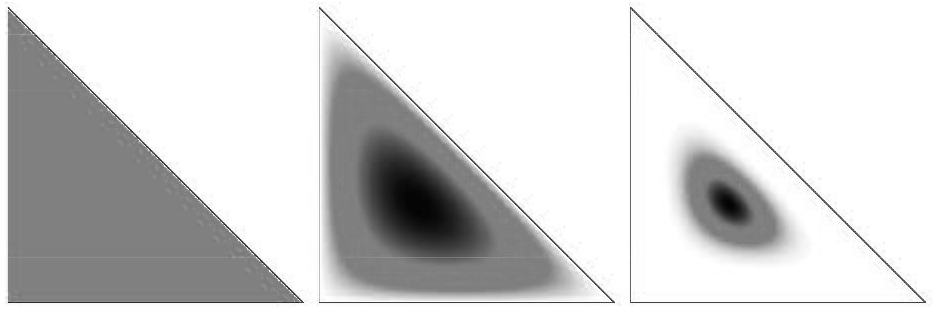
\includegraphics[width=0.6\linewidth]{topic_models/dirichlet_1} \\
\begin{tabular}{ccc}
$\vec \alpha = \left(\frac{1}{3}, \frac{1}{3}, \frac{1}{3} \right)$ &
$\vec \alpha = \left(2, 2, 2 \right)$ & 
$\vec \alpha = \left(10, 10, 10 \right)$  \\
\end{tabular} }

\only<3>{

\includegraphics[width=0.6\linewidth]{topic_models/dirichlet_2} \\
\begin{tabular}{ccc}
$\vec \alpha = \left(2, 10, 2 \right)$ & 
$\vec \alpha = \left(2, 2, 10 \right)$ & 
$\vec \alpha = \left(\frac{4}{5}, \frac{4}{5}, \frac{4}{5} \right)$  \\
\end{tabular} }

\end{center}

\end{frame}

\begin{frame}
\frametitle{Dirichlet Distribution}
\begin{center}
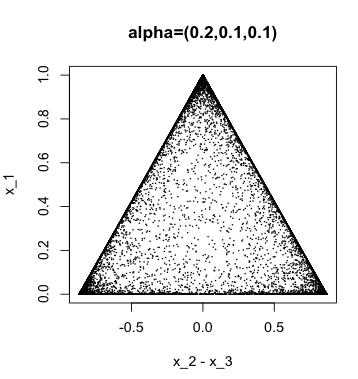
\includegraphics[width=0.5\linewidth]{topic_models/sparsity}
\end{center}
\end{frame}

\fi
\ifconjugacy

\begin{frame}
\frametitle{Dirichlet Distribution}
\begin{itemize}
  \item If ${\bm \phi} \sim \Dir(\alpha)$, ${\bm w} \sim \Mult(\phi)$, and $n_k = |\{ w_i : w_i = k\}|$ then
  \begin{align}
  	p(\phi | \alpha, {\bm w}) & \propto p({\bm w} | \phi) p(\phi | \alpha) \\
	                       & \propto  \prod_{k} \phi^{n_k} \pause  \prod_k { \phi^{\alpha_k - 1}} \\
	                       & \propto \prod_k \phi^{\alpha_k + n_k - 1}
  \end{align}
  \item Conjugacy: this {\bf posterior} has the same form as the {\bf prior}
\end{itemize}
\end{frame}

\fi

\ifhighlevel

\else

\frame
{
  \frametitle{Generative Model Approach}

\begin{center}
\only<1>{ 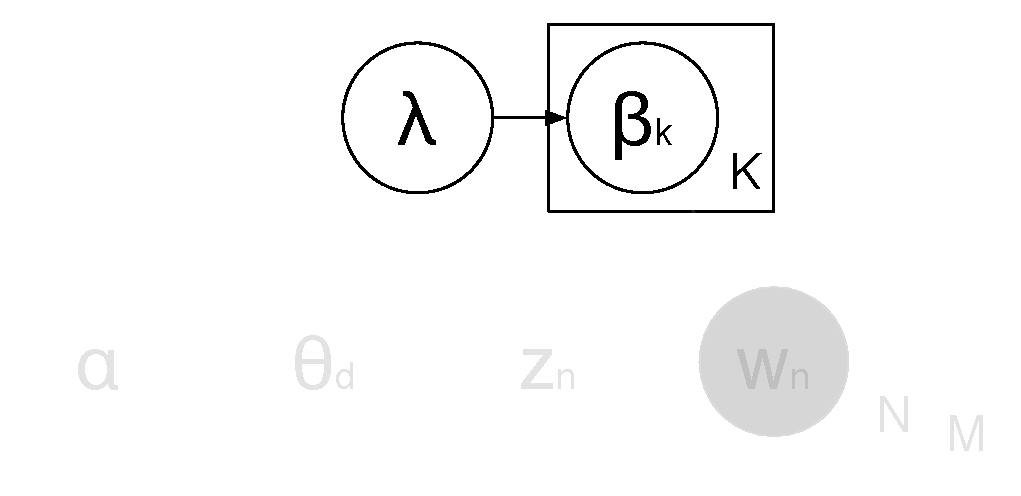
\includegraphics[scale=0.4]{topic_models/lda1.pdf} }
\only<2>{ 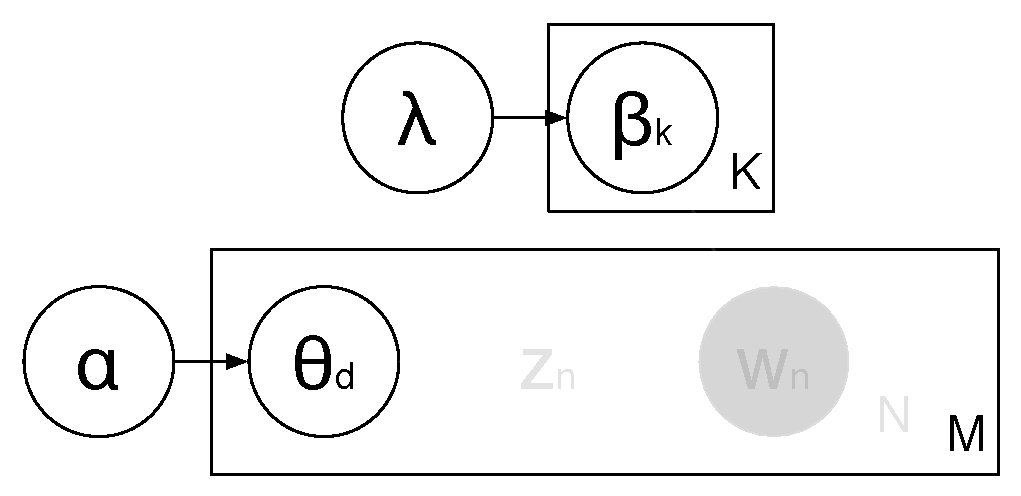
\includegraphics[scale=0.4]{topic_models/lda2.pdf} }
\only<3>{ 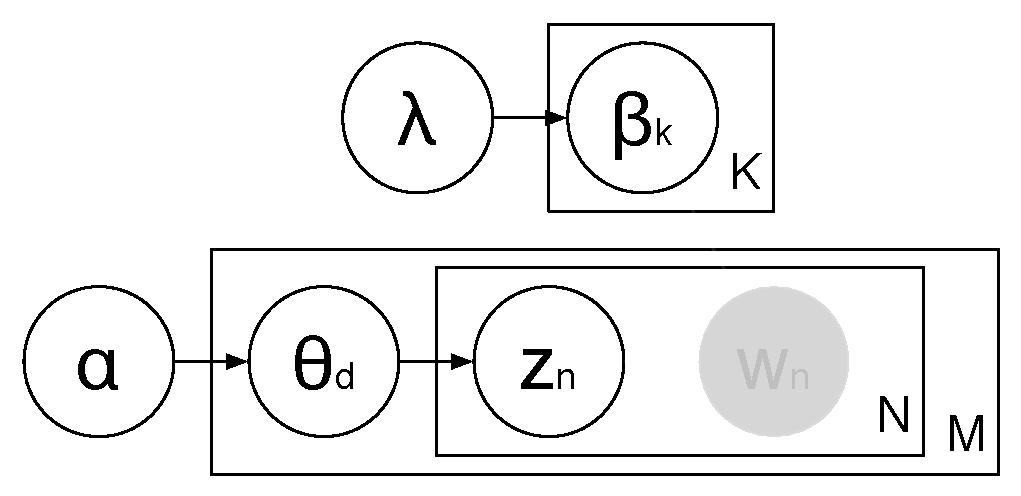
\includegraphics[scale=0.4]{topic_models/lda3.pdf} }
\only<4->{ 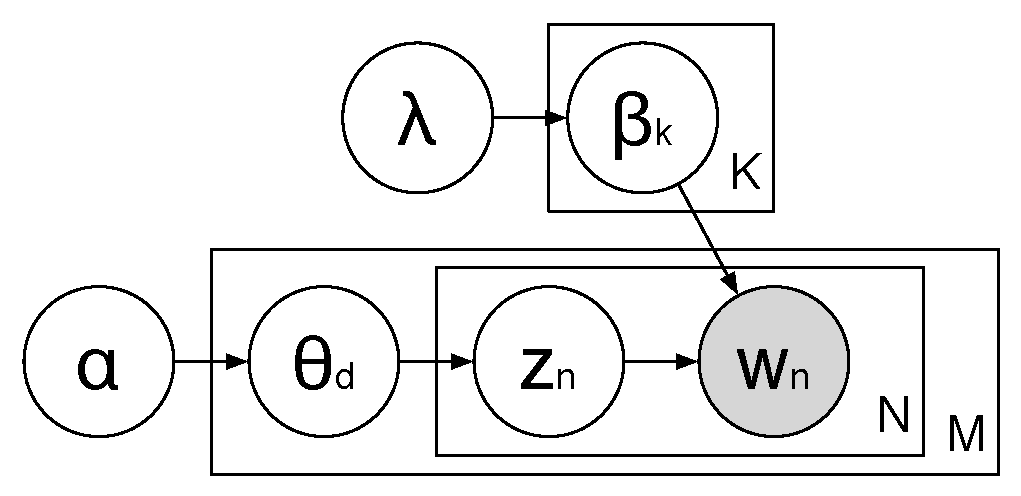
\includegraphics[scale=0.4]{topic_models/lda4.pdf} }
\end{center}

\begin{itemize}
\item<1-> For each topic $k \in \{1, \dots, K\}$, draw a multinomial distribution $\beta_k$ from a Dirichlet distribution with parameter $\lambda$
\item<2-> For each document $d \in \{1, \dots, M\}$, draw a multinomial distribution $\theta_d$ from a Dirichlet distribution with parameter $\alpha$
\item<3-> For each word position $n \in \{1, \dots, N\}$, select a hidden topic $z_n$ from the multinomial distribution parameterized by $\theta$.
\item<4-> Choose the observed word $w_n$ from the distribution $\beta_{z_n}$.
\end{itemize}

\only<5->{We use statistical inference to uncover the most likely unobserved variables given observed data.}
}

\fi

\begin{frame}
\frametitle{Topic Models: What's Important}
\begin{itemize}
\item Topic models \only<2>{(latent variables)}
\begin{itemize}
\ifhighlevel
	\item Topics to words
	\item Documents to topics
\else
	\item Topics to words---multinomial distribution
	\item Documents to topics---multinomial distribution
\fi
\end{itemize}
\item Focus in this talk: statistical methods
  \begin{itemize}
    \item Model: story of how your data came to be
    \item Latent variables: missing pieces of your story
    \item Statistical inference: filling in those missing pieces
  \end{itemize}
\item We use latent Dirichlet allocation (LDA)~\cite{blei-03}, a fully Bayesian
  version of pLSI~\cite{hofmann-99}, probabilistic version of
  LSA~\cite{landauer-97}
\end{itemize}

\end{frame}

\ifevaluation


\frame{
\frametitle{Evaluation}
\begin{center}
%\only<1>{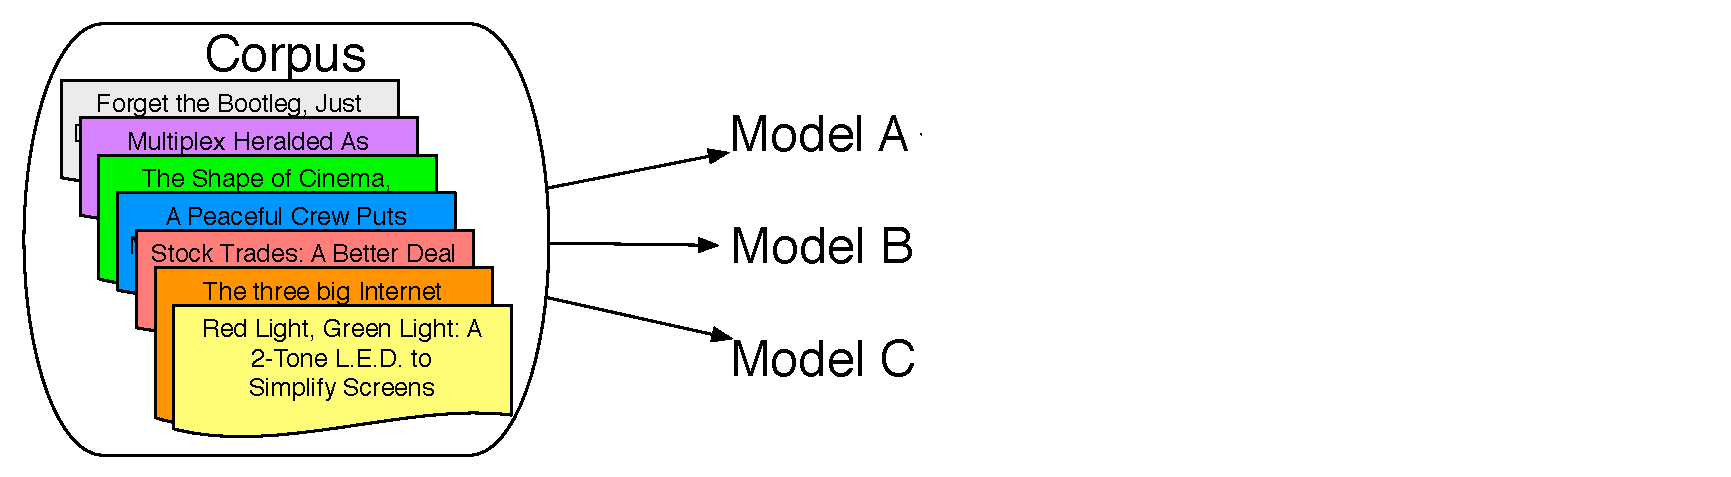
\includegraphics[width=0.9\linewidth]{reading_tea_leaves/figures/heldout_1} }
\only<1>{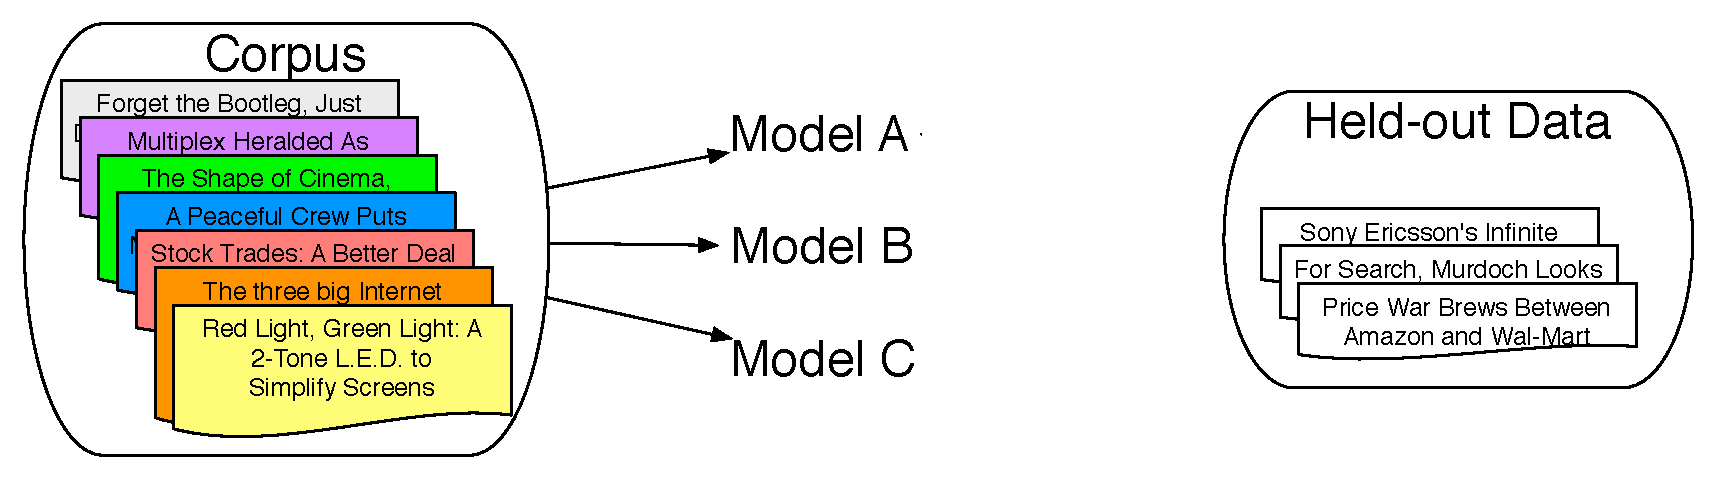
\includegraphics[width=\linewidth]{reading_tea_leaves/figures/heldout_2} }
%\only<3>{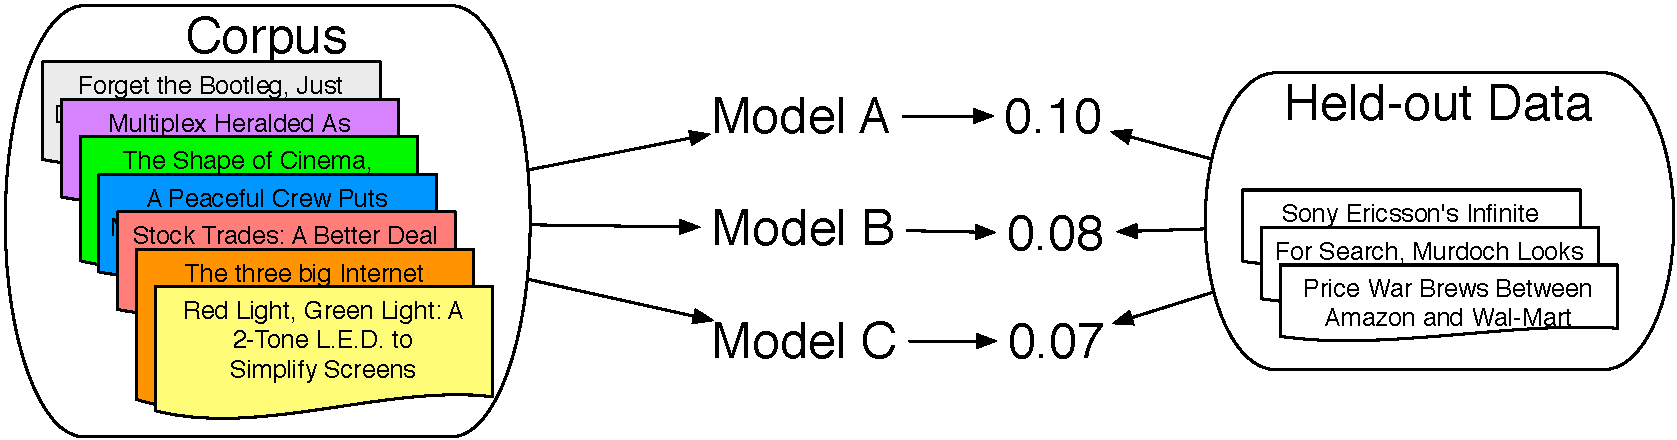
\includegraphics[width=\linewidth]{reading_tea_leaves/figures/heldout_3} }
\only<2>{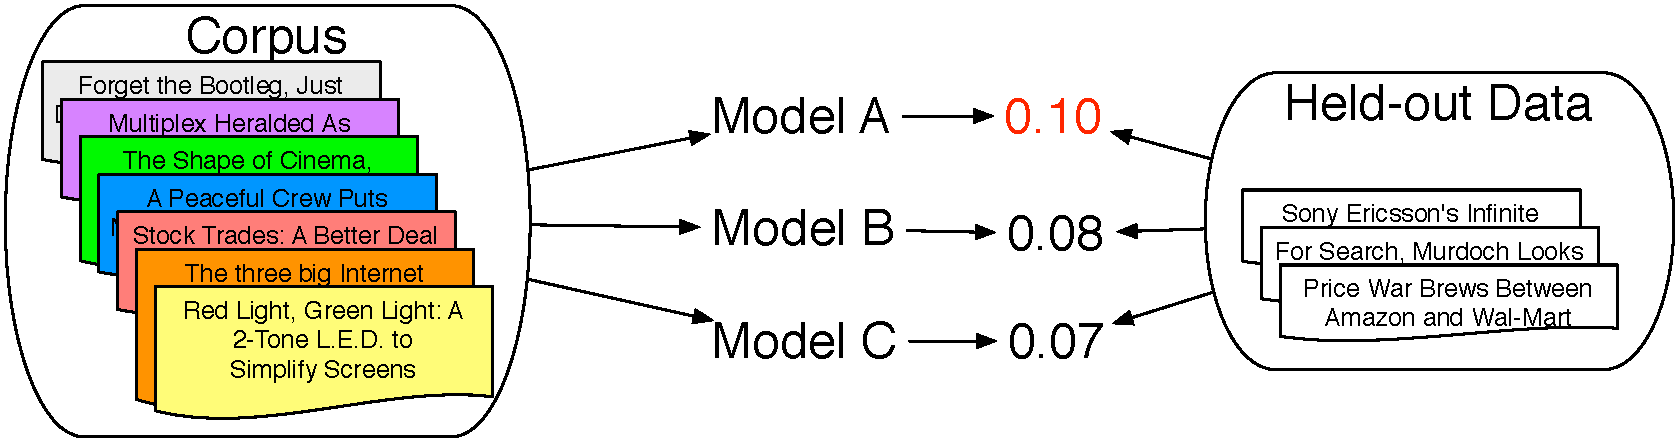
\includegraphics[width=\linewidth]{reading_tea_leaves/figures/heldout_4}  \\
	\large Measures predictive power, not what the topics are}
\end{center}

\begin{center}
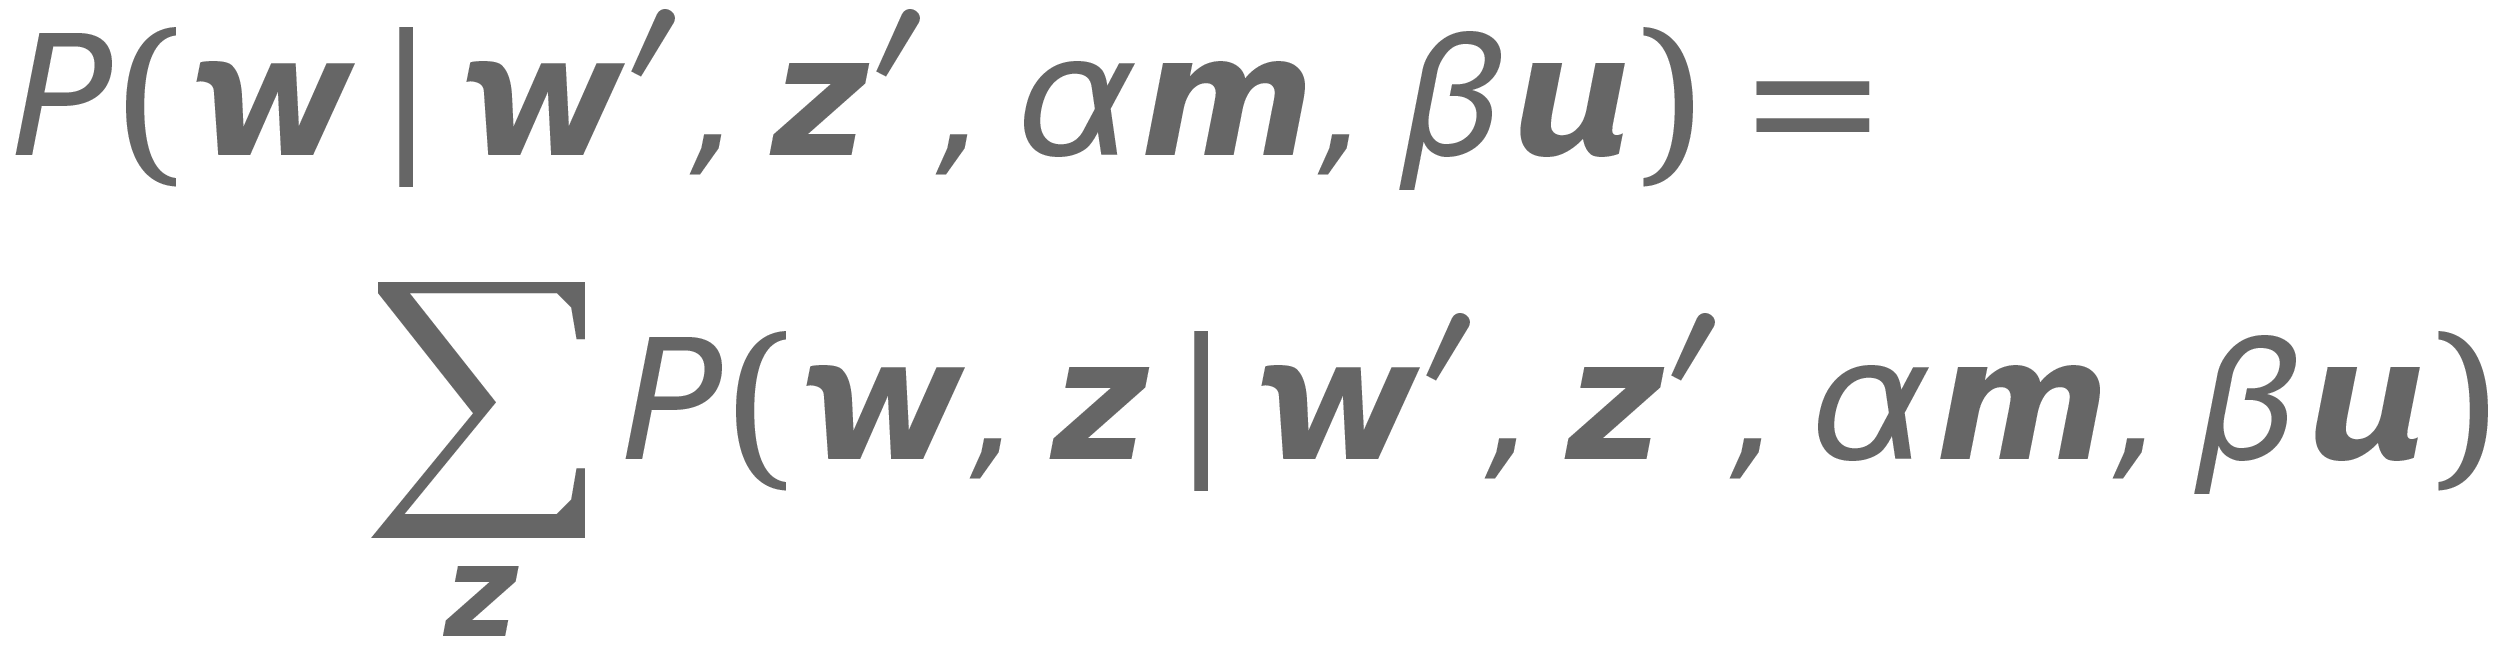
\includegraphics[width=0.5\linewidth]{topic_models/equations/evaluation} \\
How you compute it is important too~\cite{wallach-09b}
\end{center}

}

\frame{
  \frametitle{Word Intrusion}

  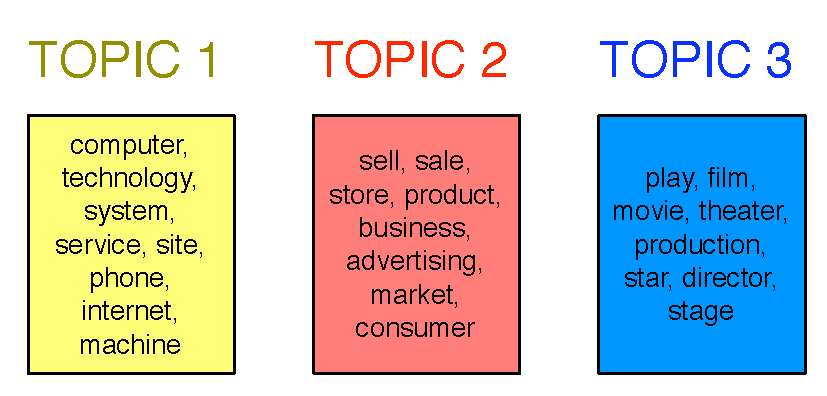
\includegraphics[width=\linewidth]{reading_tea_leaves/figures/nyt_topics_wide}
}


\frame{
  \frametitle{Word Intrusion}

  \begin{enumerate}
    \item Take the highest probability words from a topic

      \begin{block}{Original Topic}
        dog, cat, horse, pig, cow
      \end{block}
\pause
    \item Take a high-probability word from another topic and add it
      \begin{block}{Topic with Intruder}
        dog, cat, \alert<2->{apple}, horse, pig, cow
      \end{block}
\pause
     \item We ask users to find the word that doesn't belong
  \end{enumerate}
\begin{block}{Hypothesis}
If the topics are interpretable, users will consistently choose true intruder
\end{block}
}

\frame{
\frametitle{Word Intrusion}
\begin{center}
\only<1>{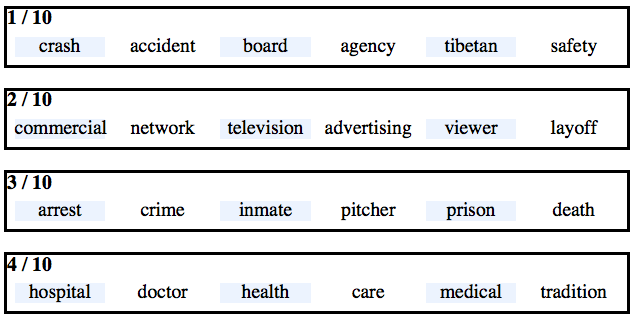
\includegraphics[width=\linewidth]{reading_tea_leaves/tasks/word1}  }
\only<2>{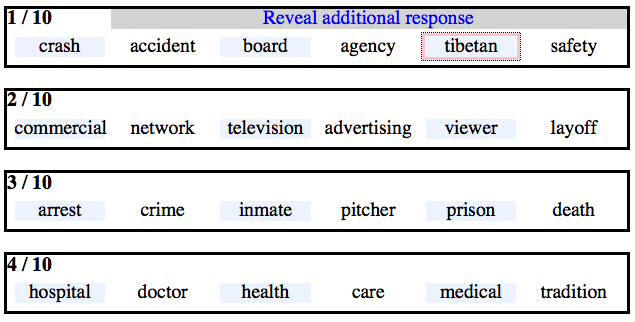
\includegraphics[width=\linewidth]{reading_tea_leaves/tasks/word2}  }
\pause
  \begin{itemize}
    \item Order of words was shuffled
    \item Which intruder was selected varied
    \item Model precision: percentage of users who clicked on intruder
  \end{itemize}

\end{center}
}

\frame{
\frametitle{Word Intrusion: Which Topics are Interpretable?}
  \begin{block}{New York Times, 50 LDA Topics}
    \begin{center}
      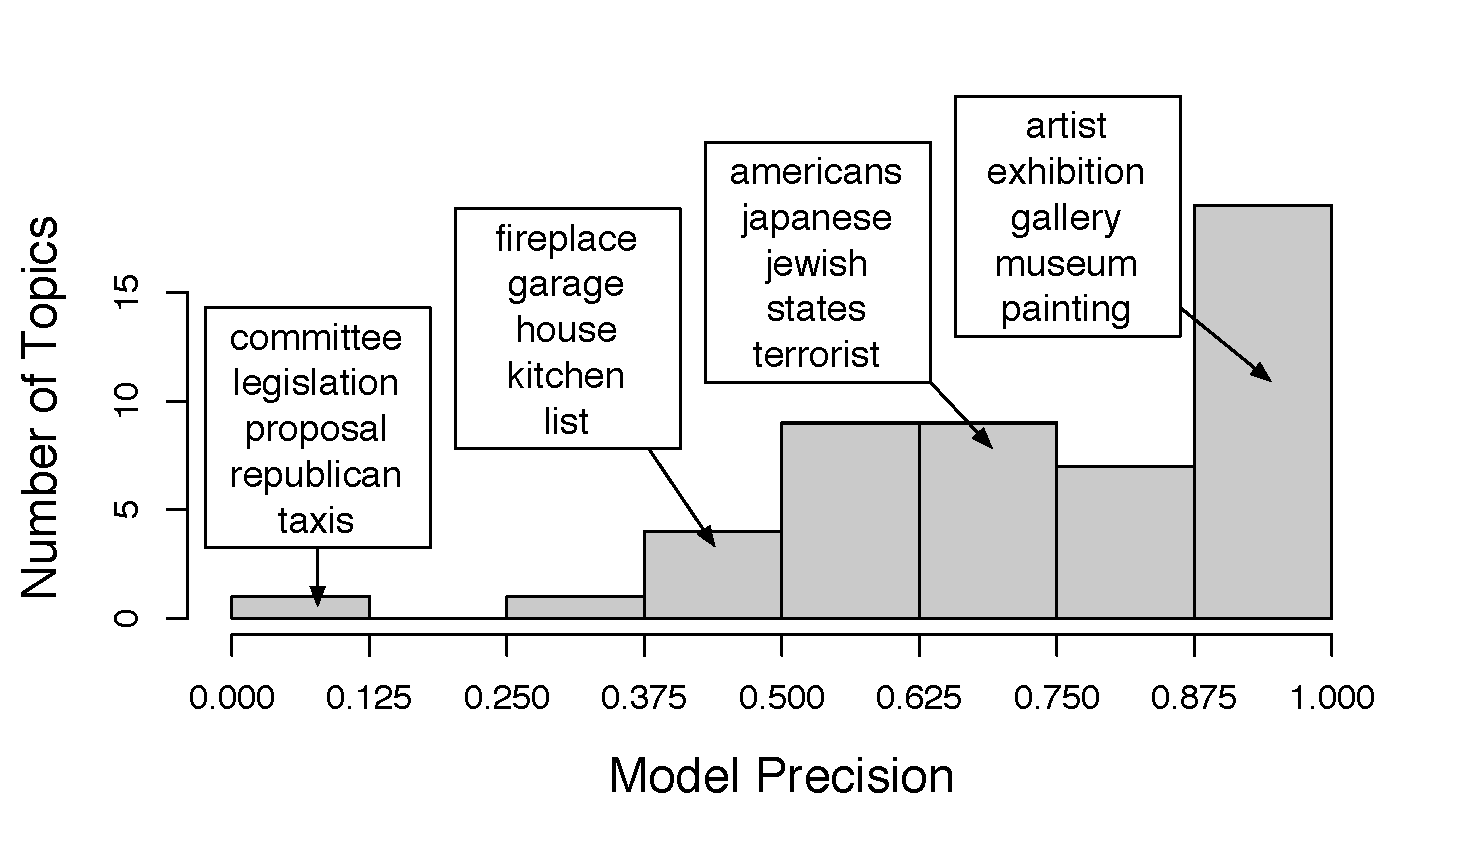
\includegraphics[width=0.8\linewidth]{reading_tea_leaves/figures/topic_precision}
    \end{center}
  \end{block}
  \begin{center}
    Model Precision: percentage of correct intruders found
  \end{center}
}



\frame{

\frametitle{Interpretability and Likelihood}
\begin{center}
\only<1>{Model Precision on New York Times}
\only<2>{Topic Log Odds on Wikipedia}
\end{center}

\begin{columns}
\column{.85\linewidth}
\begin{flushright}
  \only<1>{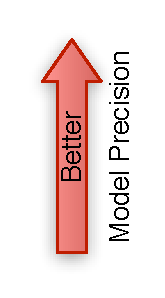
\includegraphics[scale=\graphscale]{reading_tea_leaves/tasks/mp}}
  \only<2>{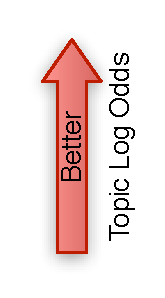
\includegraphics[scale=\graphscale]{reading_tea_leaves/tasks/tlo}}
  \only<1>{
\includegraphics[scale=\graphscale]{reading_tea_leaves/tasks/mp_y}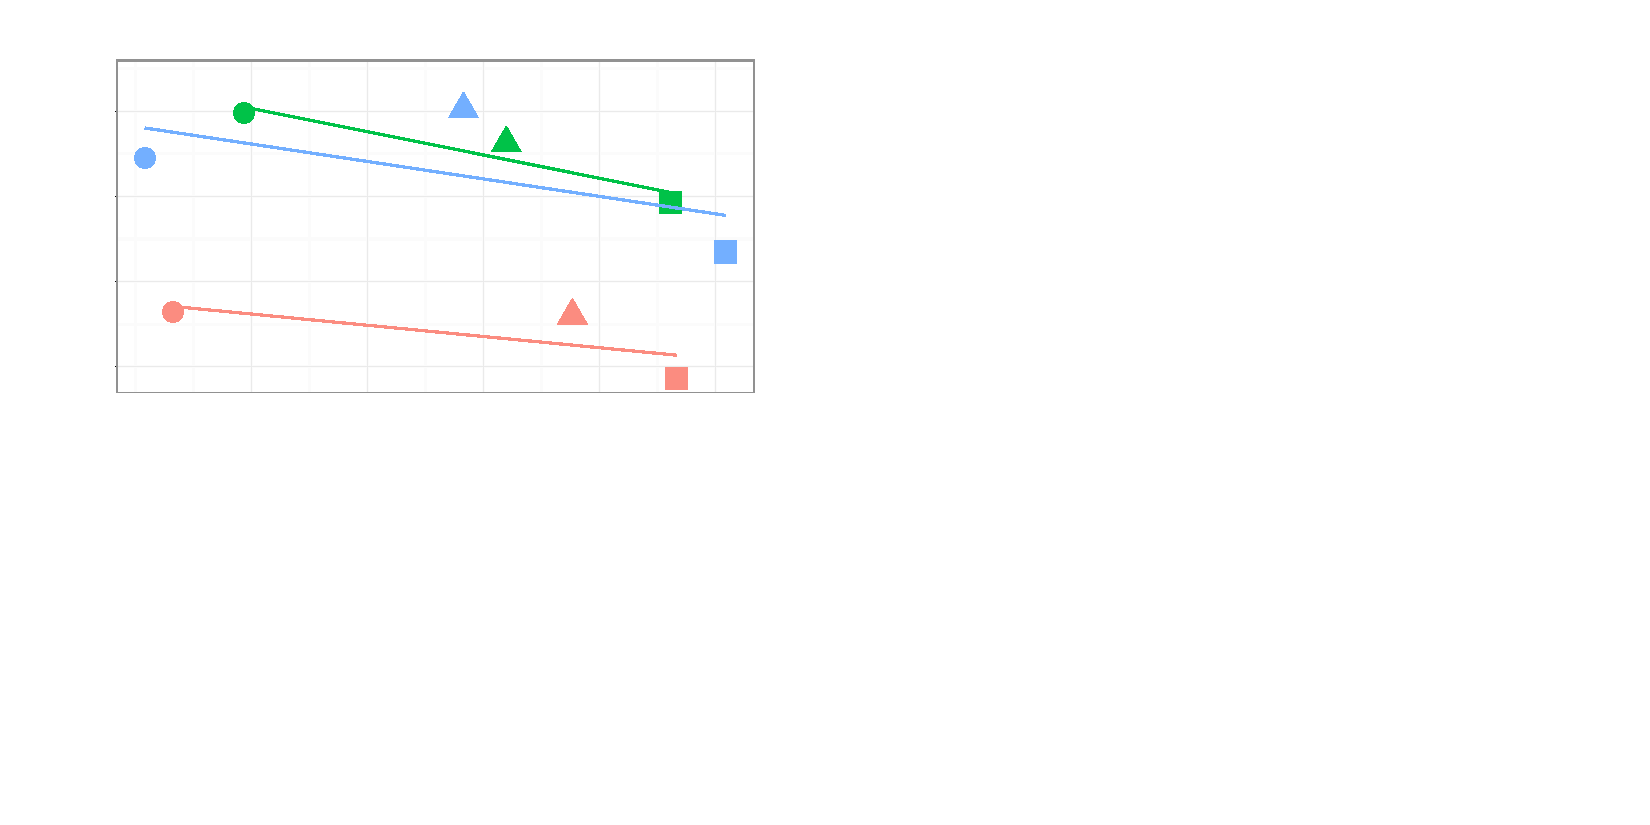
\includegraphics[scale=\graphscale]{reading_tea_leaves/tasks/nyt_mp}}
  \only<2>{
\includegraphics[scale=\graphscale]{reading_tea_leaves/tasks/tlo_y}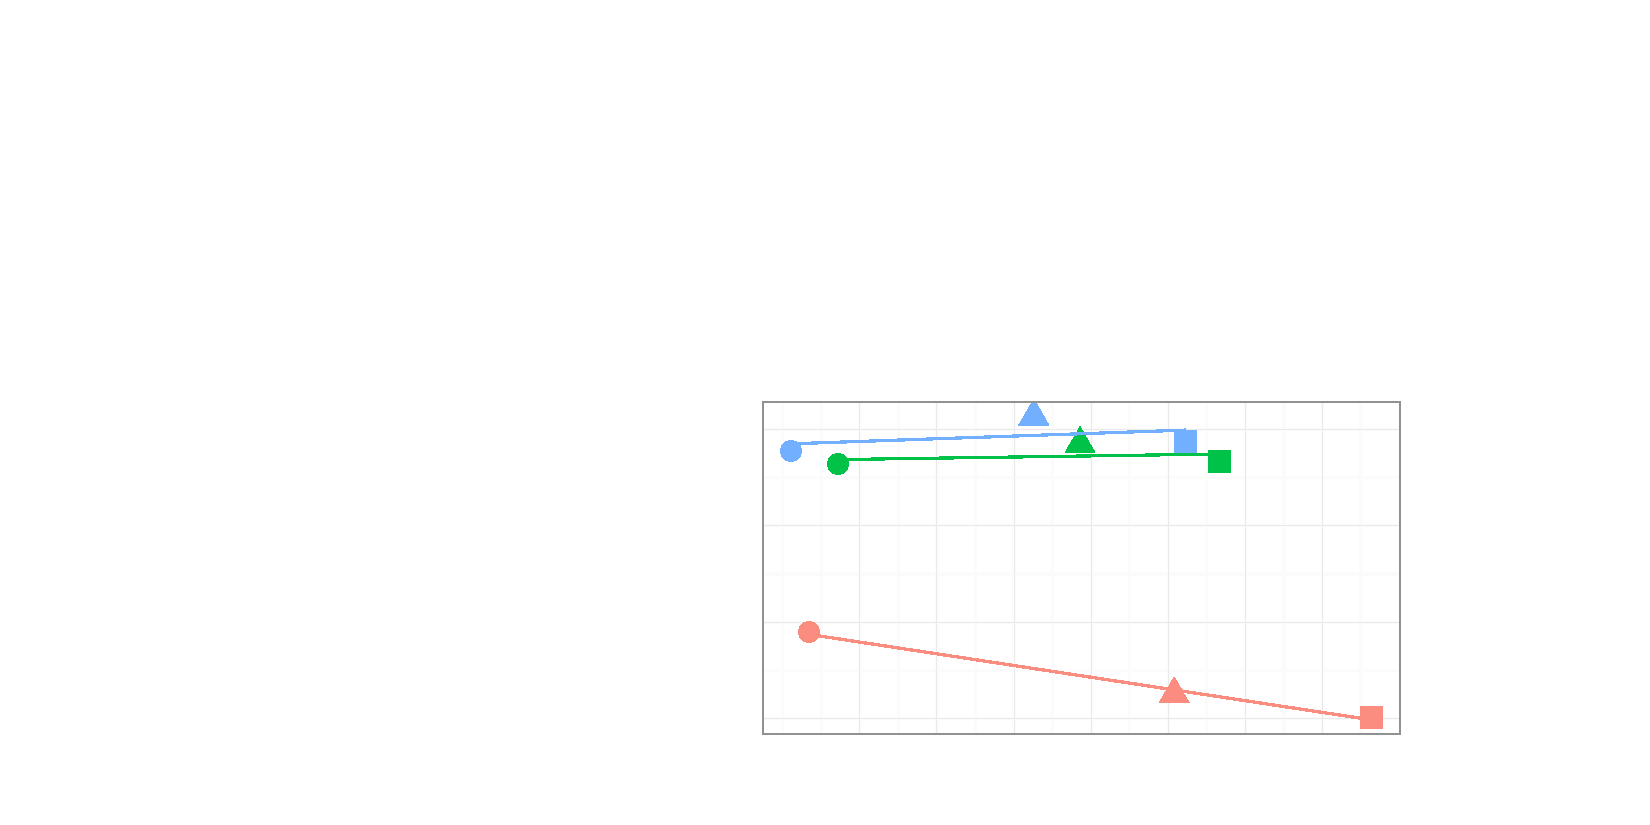
\includegraphics[scale=\graphscale]{reading_tea_leaves/tasks/wiki_tlo}} \\
  \only<1>{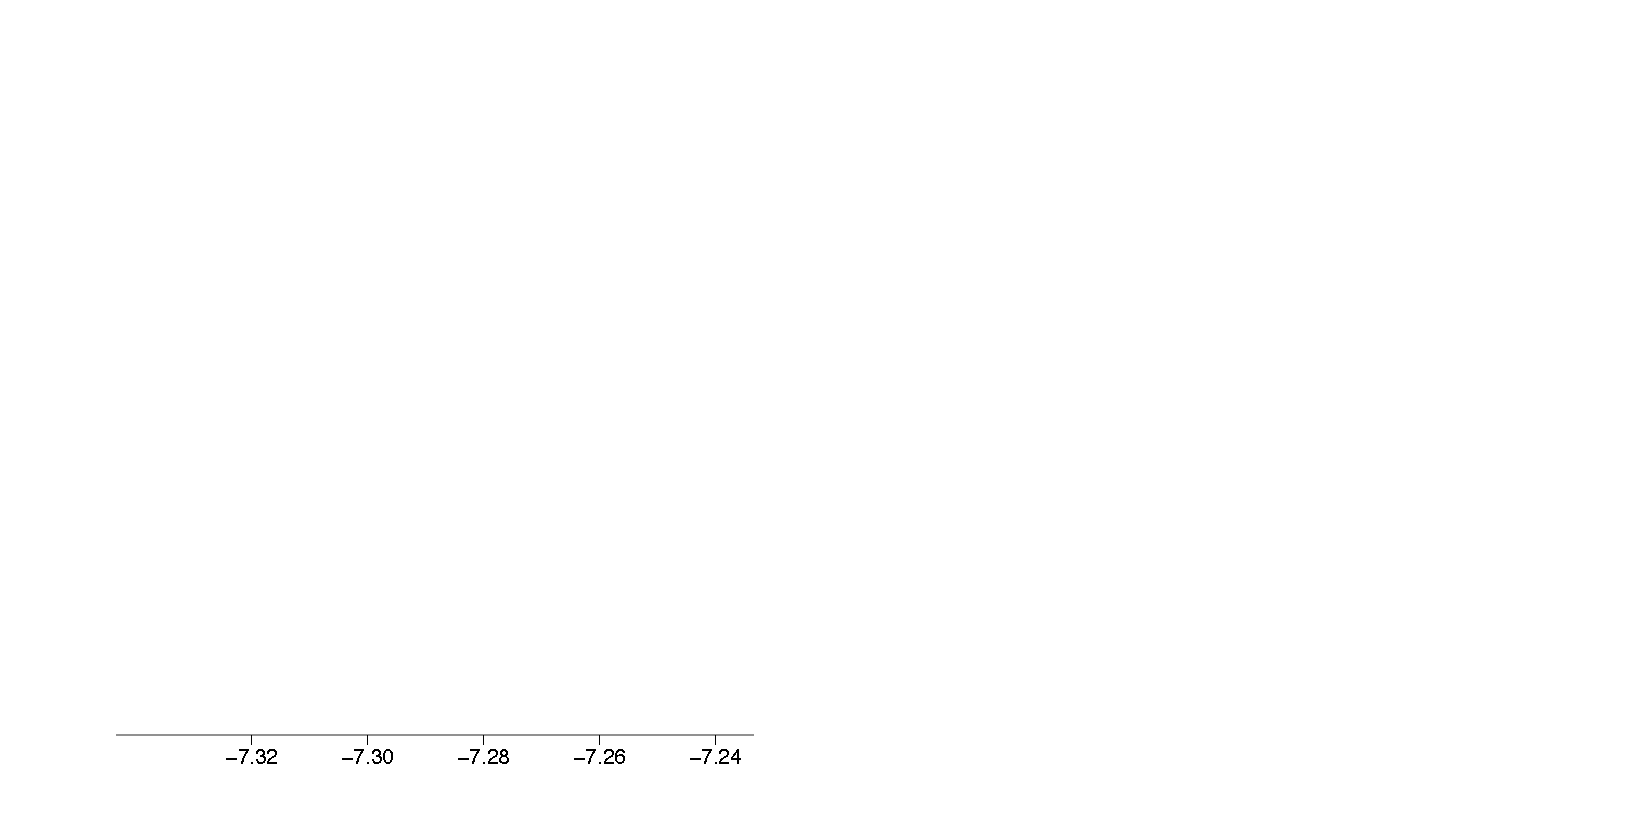
\includegraphics[scale=\graphscale]{reading_tea_leaves/tasks/nyt_x}}
  \only<2>{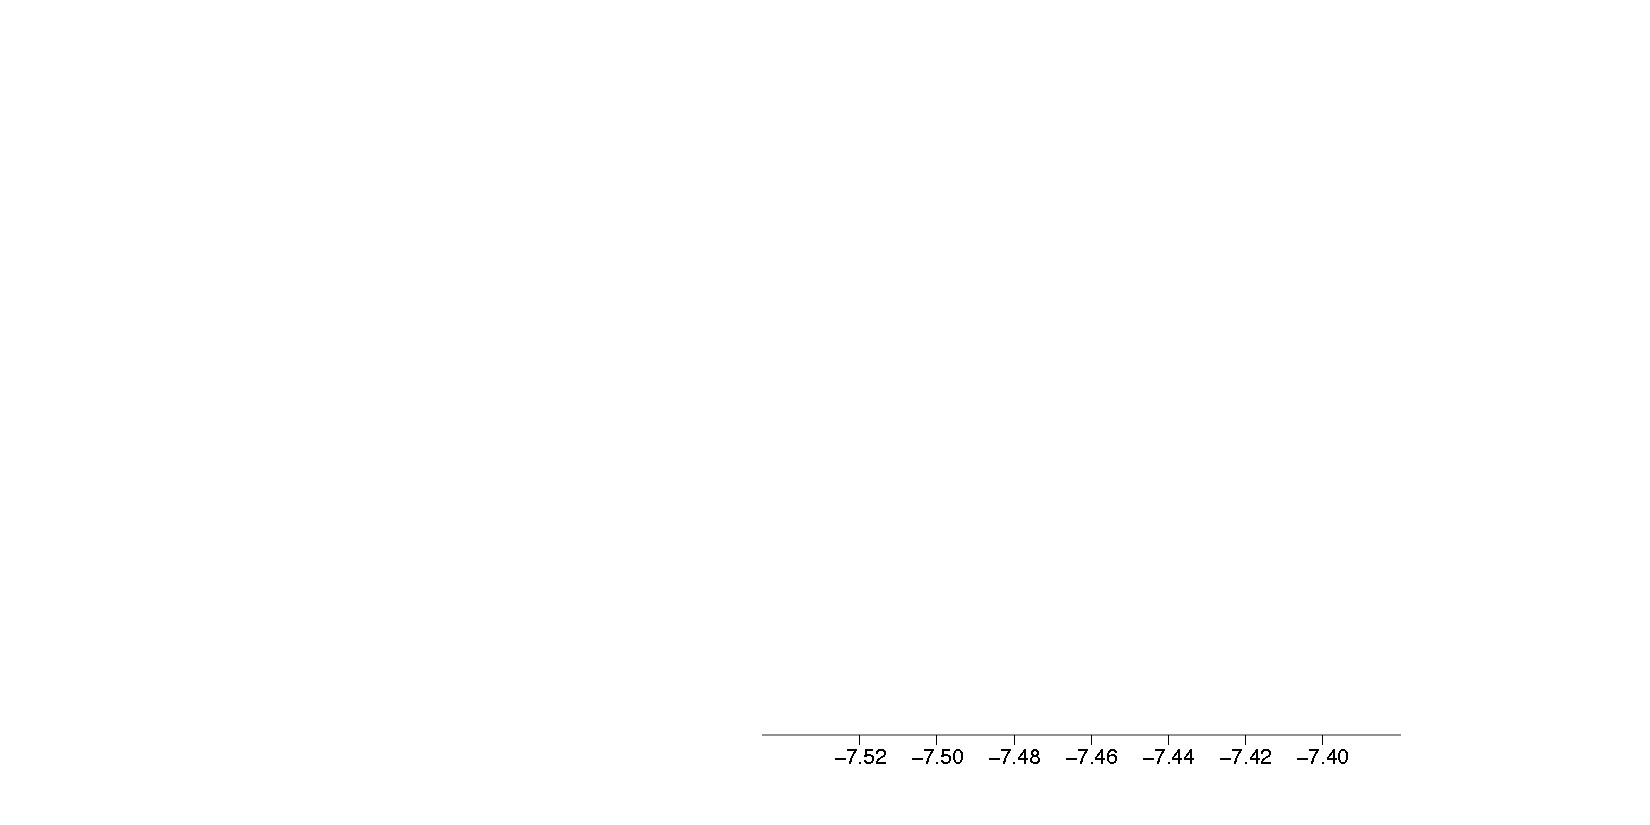
\includegraphics[scale=\graphscale]{reading_tea_leaves/tasks/wiki_x}}
\end{flushright}
\column{.15\linewidth}
  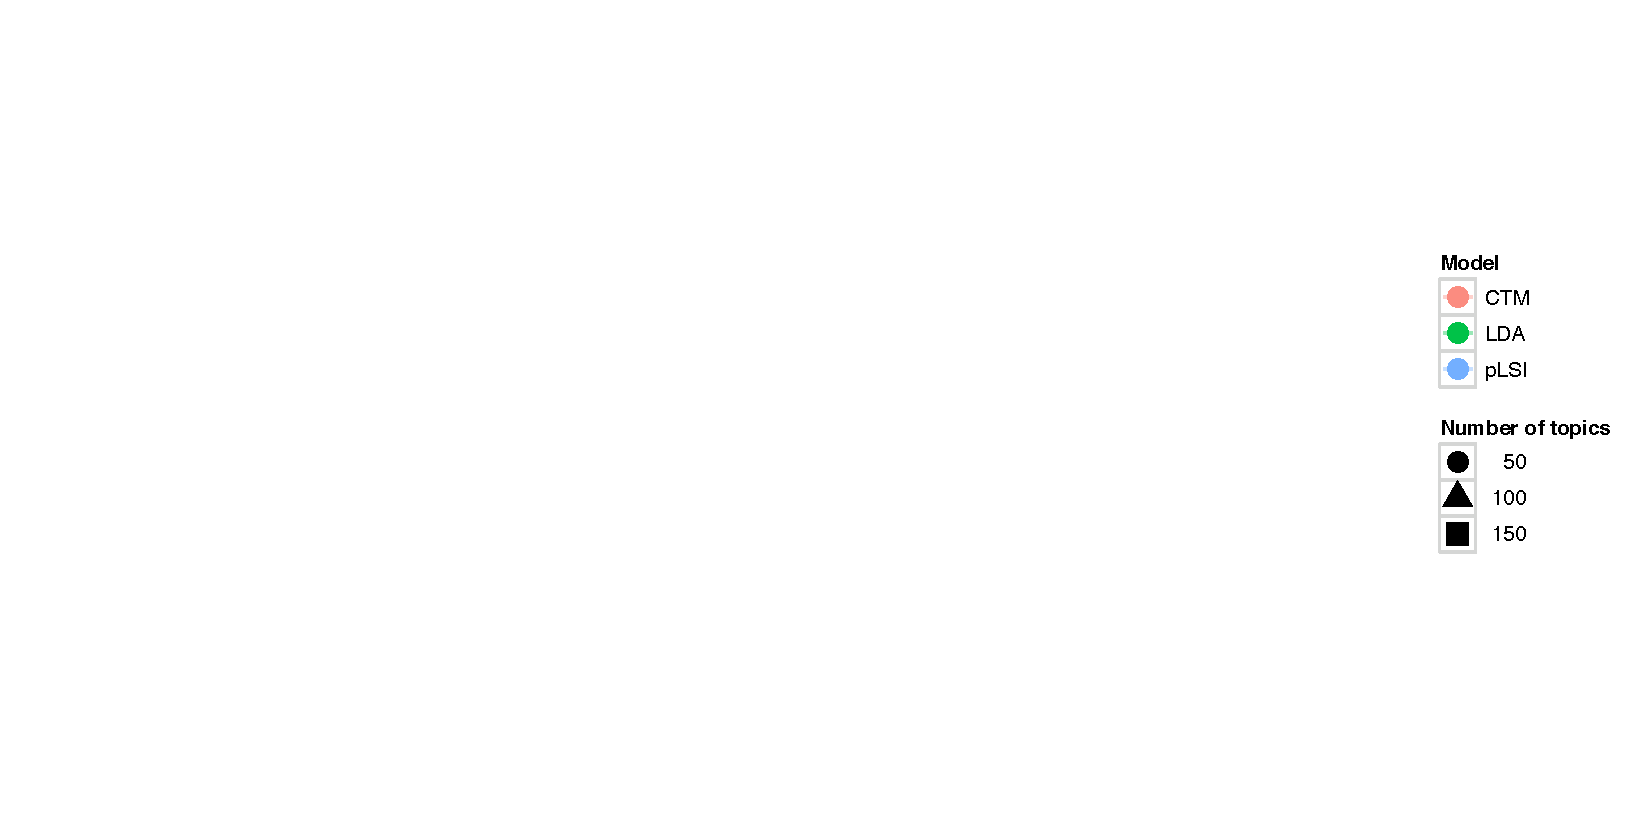
\includegraphics[scale=\graphscale]{reading_tea_leaves/tasks/legend}
\end{columns}
\vspace{-0.75cm}
\begin{center}
  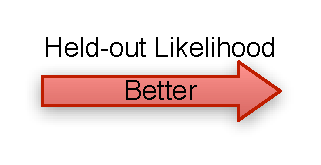
\includegraphics[scale=\graphscale]{reading_tea_leaves/tasks/held-out} \\
\only<1> {within a model, higher likelihood $\not =$ higher interpretability}
\only<2> {across models, higher likelihood $\not =$ higher interpretability}
\end{center}
}


\begin{frame}
  \frametitle{Evaluation Takeaway}

  \begin{itemize}
    \item Measure what you care about~\cite{chang-09c}
      \item If you care about prediction, likelihood is good
\item If you care about a particular task, measure that
    \end{itemize}

\end{frame}

\fi


\section{Inference}


\providecommand{\dirfunc}[3]{ \frac{ \prod_{#1}^{#2} \g{ #3 } } { \g{ \sum_{#1}^{#2} #3 }}}
\providecommand{\dirnum}[4]{ \frac{\g{ #3 }}{#4} \prod_{#1}^{#2} }
\providecommand{\dirden}[3]{ \g{ \sum_{#1}^{#2} #3 } }

\begin{frame}
\frametitle{Inference}

\begin{itemize}
\item We are interested in posterior distribution
\begin{equation}
p(Z | X, \Theta)
\end{equation}
\pause
\item Here, latent variables are topic assignments $z$ and topics $\theta$.  $X$ is the words (divided into documents), and $\Theta$ are hyperparameters to Dirichlet distributions: $\alpha$ for topic proportion, $\lambda$ for topics.
\begin{equation}
p({\bm z}, {\bm \beta}, {\bm \theta} | {\bm w}, \alpha, \lambda)
\end{equation}
\pause
\begin{align*}
p({\bm w}, {\bm z}, {\bm \theta}, {\bm \beta} & | \alpha, \lambda) = \\
& \prod_{k} p(\beta_k | \lambda) \prod_{d} p(\theta_d | \alpha) \prod_{n}
p(z_{d,n} | \theta_d) p(w_{d,n} | \beta_{z_{d,n}})
\end{align*}
\end{itemize}
\end{frame}



\begin{frame}
\frametitle{Gibbs Sampling}
\begin{itemize}
\item A form of Markov Chain Monte Carlo
\item Chain is a sequence of random variable states
\item Given a state $\{z_1, \dots z_N\}$ given certain technical conditions, drawing $z_k \sim p(z_1, \dots z_{k-1}, z_{k+1}, \dots z_N | X, \Theta)$ for all $k$ (repeatedly) results in a Markov Chain whose stationary distribution \emph{is} the posterior.
\item For notational convenience, call ${\bm z}$ with $z_{d,n}$ removed ${\bm z}_{-d,n}$
\end{itemize}
\end{frame}

\frame{
	\frametitle{Inference}
	\begin{center}
\only<1> {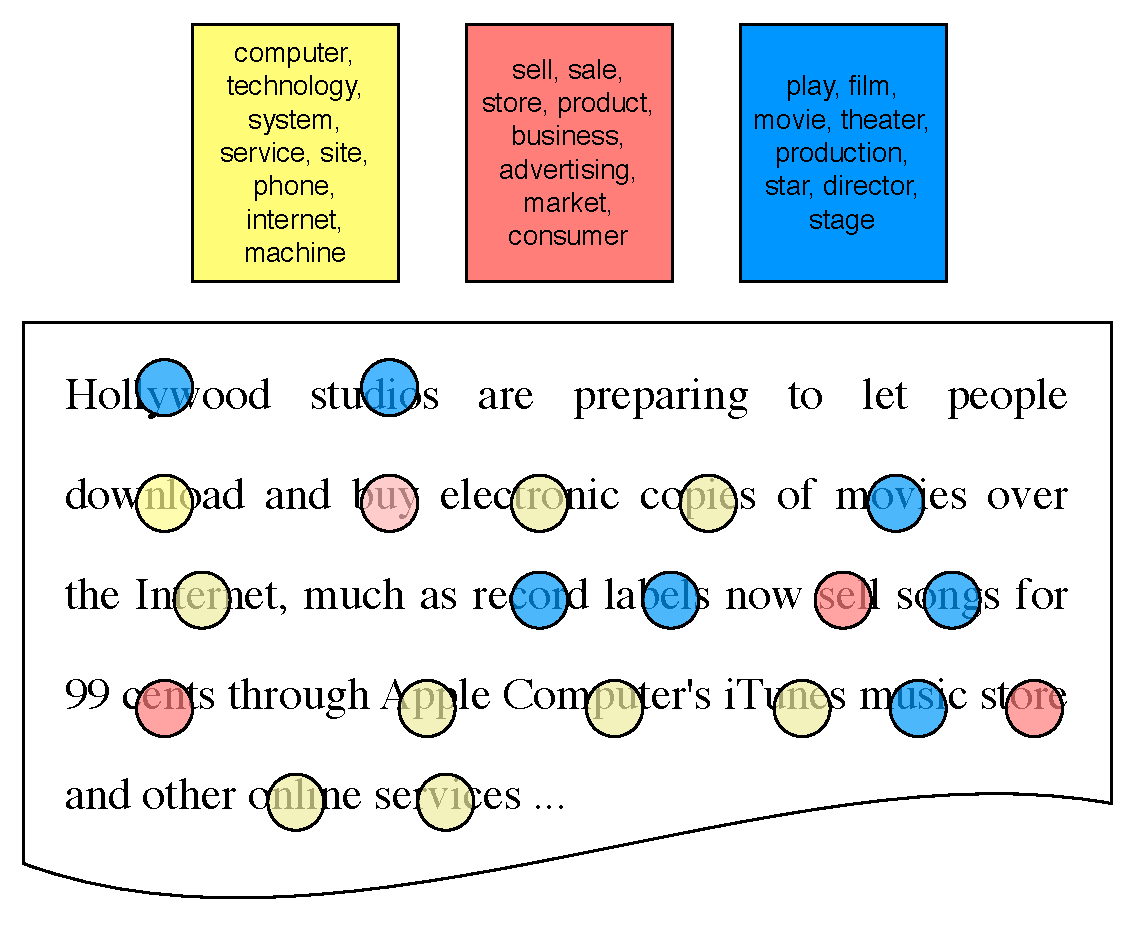
\includegraphics[width=.8\linewidth]{topic_models/inference_3}}
\only<2> {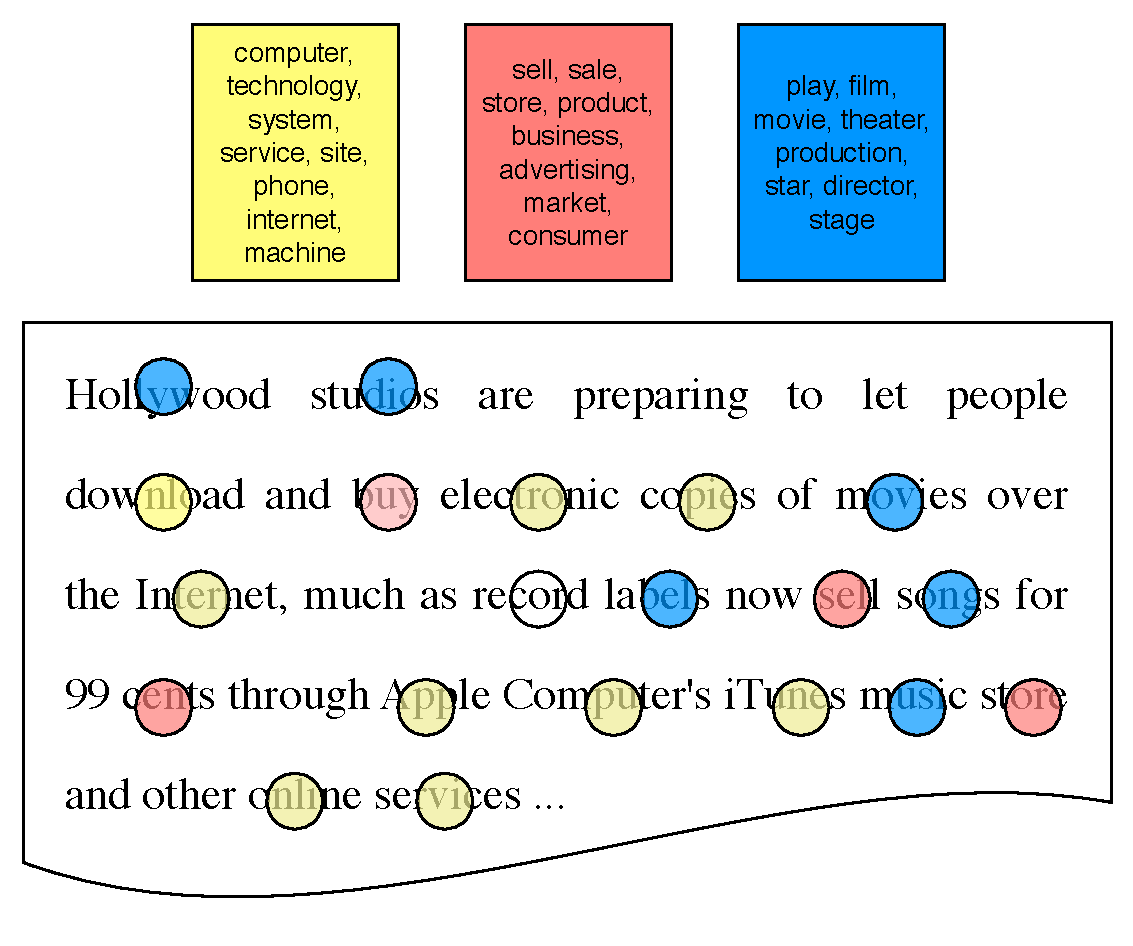
\includegraphics[width=.8\linewidth]{topic_models/inference_4}}
\only<3> {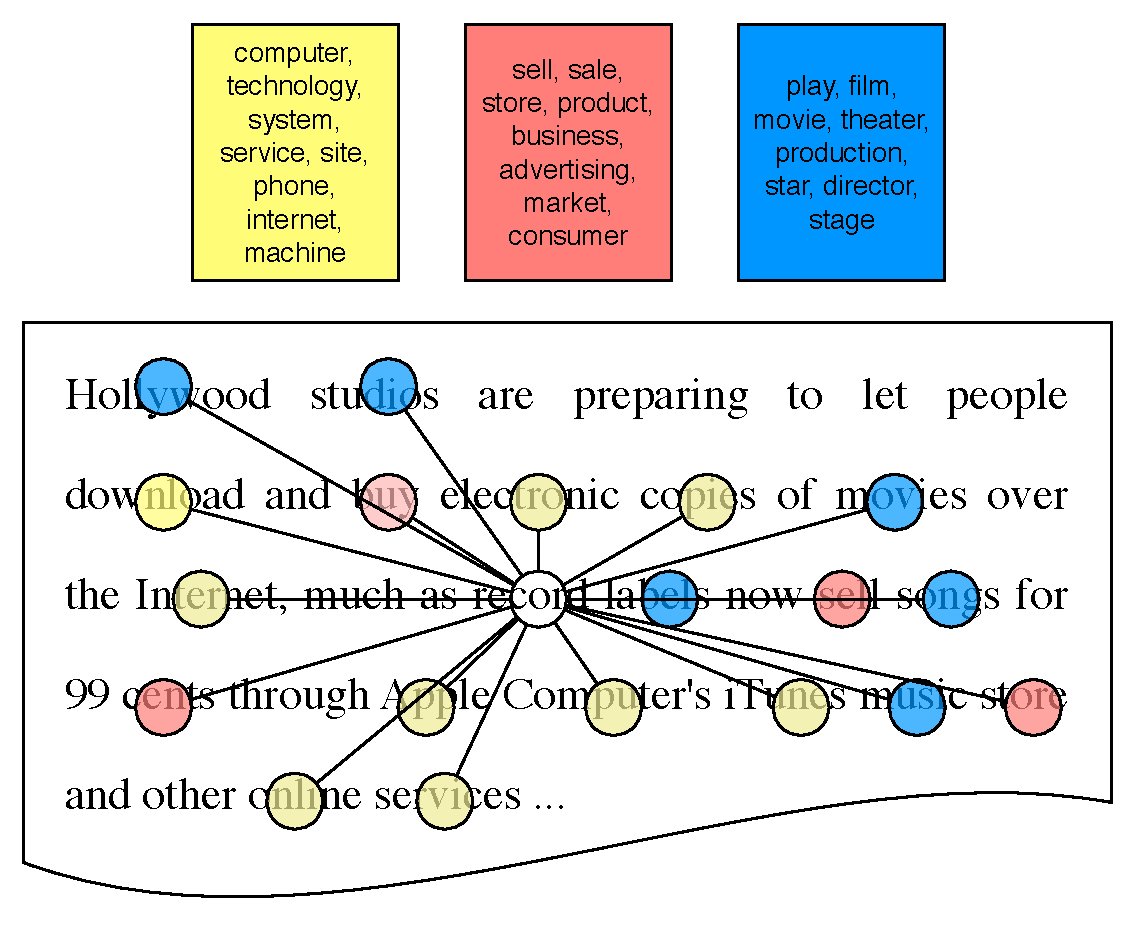
\includegraphics[width=.8\linewidth]{topic_models/inference_5}}
\only<4> {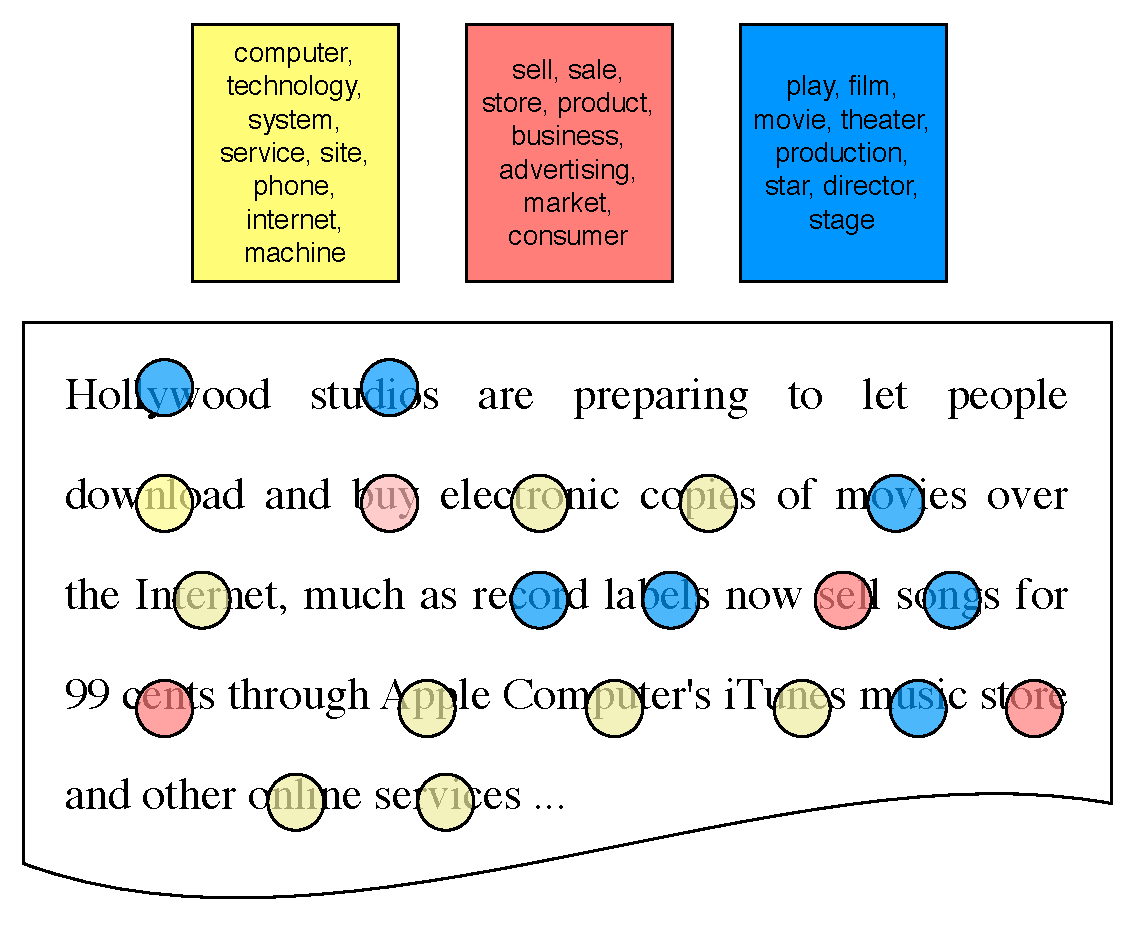
\includegraphics[width=.8\linewidth]{topic_models/inference_3}}
\only<5> {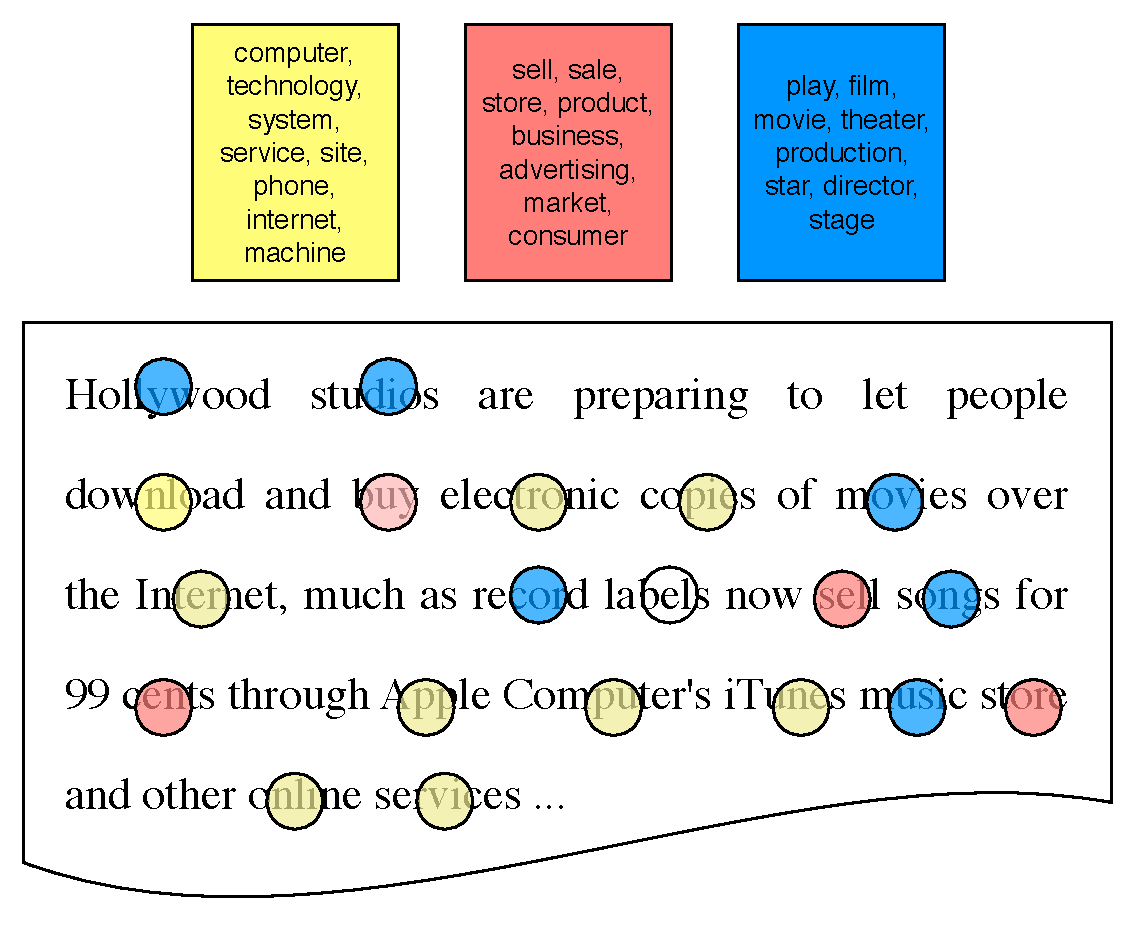
\includegraphics[width=.8\linewidth]{topic_models/inference_6}}
\only<6> {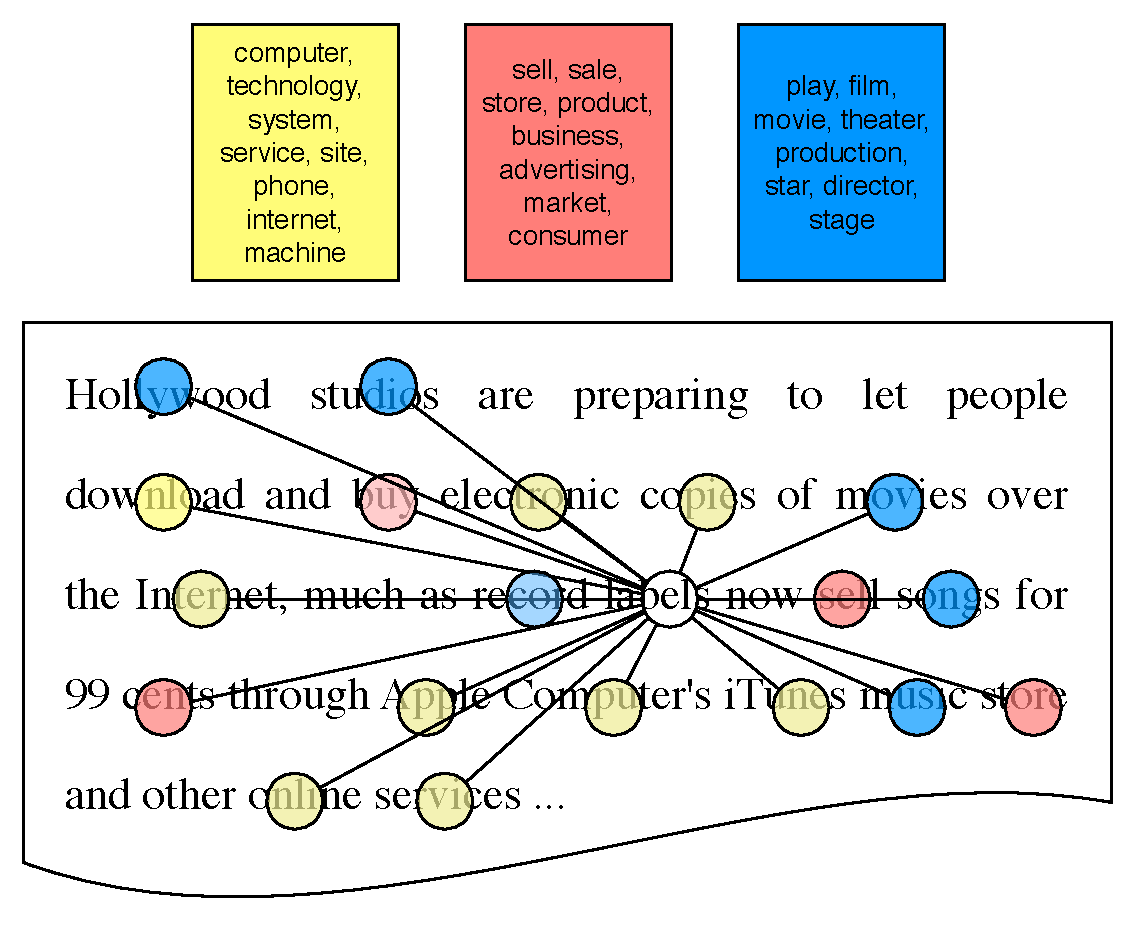
\includegraphics[width=.8\linewidth]{topic_models/inference_7}}
\only<7> {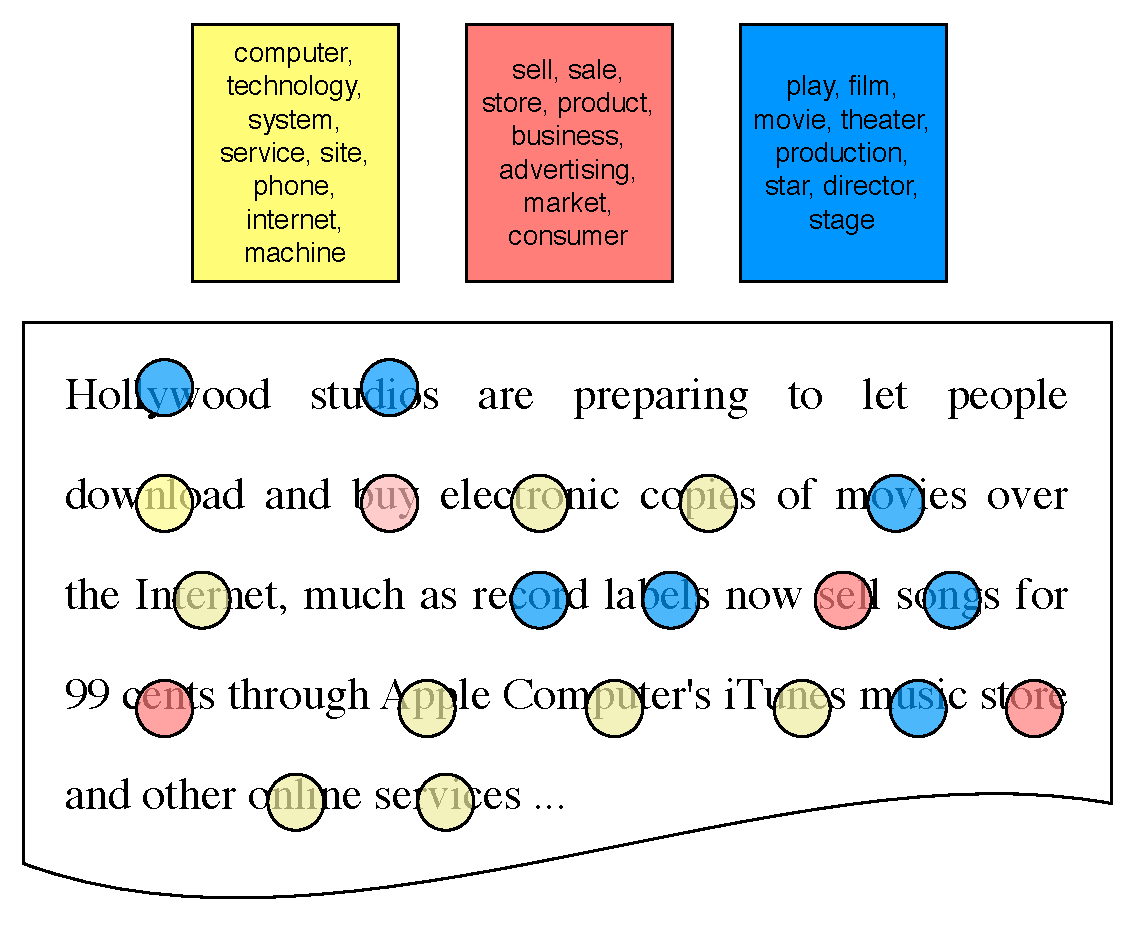
\includegraphics[width=.8\linewidth]{topic_models/inference_3}}
	\end{center}
}


\ifconjugacy

\begin{frame}
\frametitle{Gibbs Sampling}
\begin{itemize}
\item For LDA, we will sample the topic assignments
\item Thus, we want:
\begin{equation*}
p(z_{d,n} = k | {\bm z}_{-d,n}, {\bm w}, \alpha, \lambda) = \frac{ p(z_{d,n} = k, {\bm z}_{-d,n} | {\bm w}, \alpha, \lambda)} { p({\bm z}_{-d,n} | {\bm w},\alpha, \lambda)}
\end{equation*}
\pause
\item The topics and per-document topic proportions are integrated out / marginalized
\item Let $n_{d,i}$ be the number of words taking topic $i$ in document $d$.  Let $v_{k,w}$ be the number of times word $w$ is used in topic $k$.
\end{itemize}


\begin{equation*}
= \frac{ \int_{\theta_d} \left( \prod_{i \not = k} \theta_d^{\alpha_i + n_{d,i} - 1} \right)\theta_d^{\alpha_k + n_{d,i} } d\theta_d \int_{\beta_{k}}    \left( \prod_{i \not = w_{d,n}} \beta_{k,i} ^{ \lambda_i + v_{k,i} - 1} \right) \beta_{k, w_{d,n}}^{\lambda_i + v_{k,i}} d\beta_k } { \int_{\theta_d} \left( \prod_{i} \theta_d^{\alpha_i + n_{d,i} - 1} \right) d\theta_d \int_{\beta_{k}}    \left( \prod_{i} \beta_{k,i} ^{ \lambda_i + v_{k,i} - 1} \right) d\beta_k }
\end{equation*}
\end{frame}

\else

\begin{frame}
\frametitle{Gibbs Sampling}
\begin{itemize}
\item For LDA, we will sample the topic assignments
\item The topics and per-document topic proportions are integrated out / marginalized / Rao-Blackwellized
\item Thus, we want:
\begin{equation*}
p(z_{d,n} = k | {\bm z}_{-d,n}, {\bm w}, \alpha, \lambda) = \frac{n_{d, k} + \alpha_k}{ \sum_{i}^{K} { n_{d,i} + \alpha_i}} \frac{v_{k, w_{d,n}} + \lambda_{w_{d,n}}}{ \sum_{i} { v_{k,i} + \lambda_{i} }}
\end{equation*}
\end{itemize}
\end{frame}

\fi



\ifconjugacy

\begin{frame}
\frametitle{Gibbs Sampling}
\begin{itemize}
\item Integral is normalizer of Dirichlet distribution
\begin{equation*}
\int_{\beta_{k}}    \left( \prod_{i} \beta_{k,i} ^{ \lambda_i + v_{k,i} - 1} \right) d\beta_k = \dirfunc{i}{V}{\beta_i + v_{k,i}}
\end{equation*}
\pause
\item So we can simplify
\end{itemize}
\begin{footnotesize}
\begin{align*}
& \frac{ \int_{\theta_d} \left( \prod_{i \not = k} \theta_d^{\alpha_i + n_{d,i}
      - 1} \right)\theta_d^{\alpha_k + n_{d,i} } d\theta_d \int_{\beta_{k}}
  \left( \prod_{i \not = w_{d,n}} \beta_{k,i} ^{ \lambda_i + v_{k,i} - 1}
  \right) \beta_{k, w_{d,n}}^{\lambda_i + v_{k,i}} d\beta_k } { \int_{\theta_d}
  \left( \prod_{i} \theta_d^{\alpha_i + n_{d,i} - 1} \right) d\theta_d
  \int_{\beta_{k}}    \left( \prod_{i} \beta_{k,i} ^{ \lambda_i + v_{k,i} - 1}
  \right) d\beta_k } = \\
& \frac{
  \dirnum{i \not = k}{K}{\alpha_k + n_{d,k} + 1}{ \g{\sum_{i}^{K} \alpha_i +
      n_{d,i} + 1} } \g{\alpha_k + n_{d,k}}  }
{ \dirfunc{i}{K}{\alpha_i + n_{d,i}} }
% -----------------------------------
\frac{
 \dirnum{i \not = w_{d,n}}{V}{\lambda_{w_{d,n}} + v_{k,w_{d,n}} + 1}{ \g{\sum_{i}^{V} \lambda_i + v_{k,i} + 1} } \g{\lambda_k + v_{k,w_{d,n}}}
}{ \dirfunc{i}{V}{\lambda_i + v_{k,i}} } \\
% -----------------------------------
\end{align*}
\end{footnotesize}
\end{frame}


\begin{frame}

\begin{block}{Gamma Function Identity}
	\begin{equation}
		z = \frac{\Gamma(z + 1)}{\Gamma(z)}
	\end{equation}
\end{block}

\begin{footnotesize}
\begin{align*}
& \frac{
  \dirnum{i \not = k}{K}{\alpha_k + n_{d,k} + 1}{ \g{\sum_{i}^{K} \alpha_i +
      n_{d,i} + 1} } \g{\alpha_k + n_{d,k}}  }
{ \dirfunc{i}{K}{\alpha_i + n_{d,i}} }
% -----------------------------------
\frac{
 \dirnum{i \not = w_{d,n}}{V}{\lambda_{w_{d,n}} + v_{k,w_{d,n}} + 1}{ \g{\sum_{i}^{V} \lambda_i + v_{k,i} + 1} } \g{\lambda_k + v_{k,w_{d,n}}}
}{ \dirfunc{i}{V}{\lambda_i + v_{k,i}} } \\
% -----------------------------------
& = \frac{n_{d, k} + \alpha_k}{ \sum_{i}^{K} { n_{d,i} + \alpha_i}} \frac{v_{k, w_{d,n}} + \lambda_{w_{d,n}}}{ \sum_{i} { v_{k,i} + \lambda_{i} }}
\end{align*}
\end{footnotesize}

\end{frame}
\else
\fi

\begin{frame}{Gibbs Sampling Equation}
  
\begin{equation}
\alert<5>{\frac{\alert<1>{n_{d, k}} +  \alert<3>{\alpha_k}}{ \sum_{i}^{K} { n_{d,i} +\alpha_i}}} \alert<6>{\frac{\alert<2>{v_{k, w_{d,n}}} + \alert<4>{\lambda_{w_{d,n}}}}{ \sum_{i} { v_{k,i} + \lambda_{i} }}}
\end{equation}

\begin{itemize}
  \item \alert<1>{Number of times document $d$ uses topic $k$}
  \item \alert<2>{Number of times topic $k$ uses word type $w_{d,n}$}
  \item \alert<3>{Dirichlet parameter for document to topic
      distribution}
  \item \alert<4>{Dirichlet parameter for topic to word distribution}
  \item \alert<5>{How much this document likes topic $k$}
  \item \alert<6>{How much this topic likes word $w_{d,n}$}
\end{itemize}

\end{frame}

\begin{frame}
  \frametitle{Sample Document}
    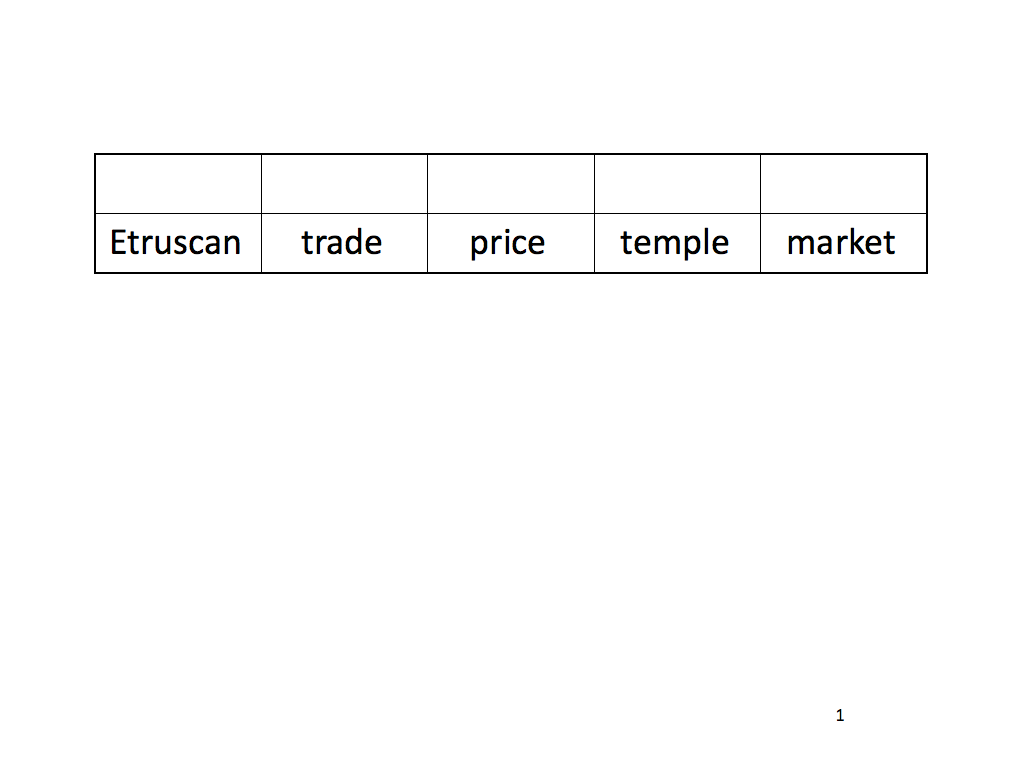
\includegraphics[width=\linewidth]{topic_models/mimno_001}
\end{frame}

\begin{frame}
  \frametitle{Sample Document}
    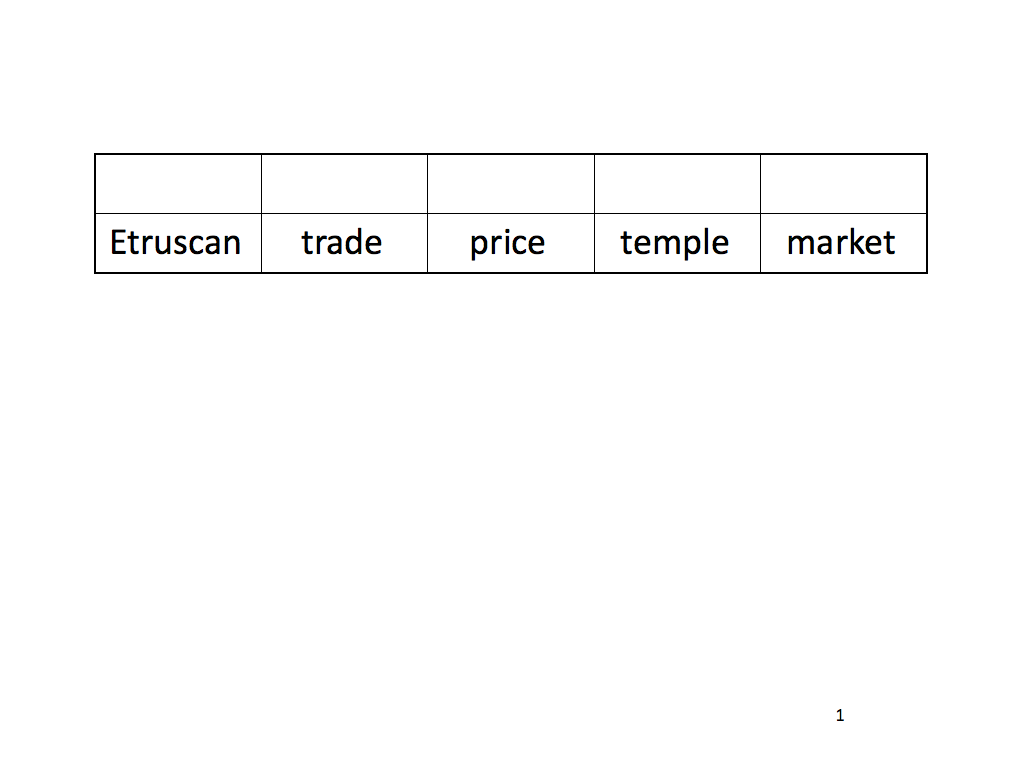
\includegraphics[width=\linewidth]{topic_models/mimno_001}
\end{frame}

\begin{frame}
  \frametitle{Randomly Assign Topics}
    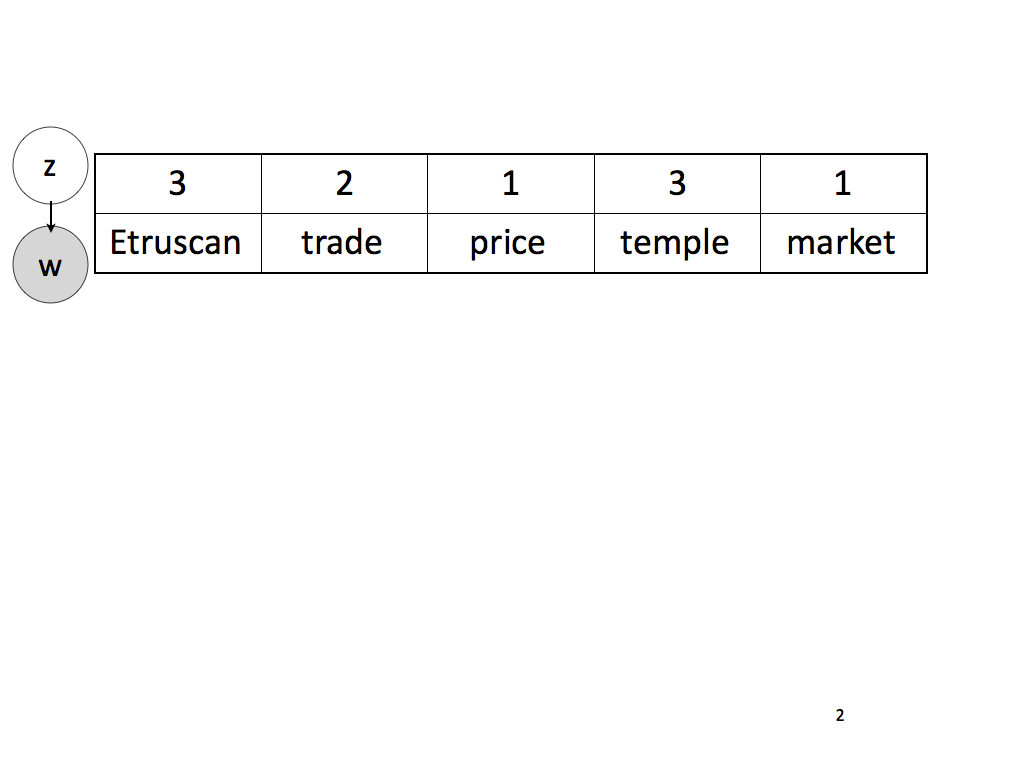
\includegraphics[width=\linewidth]{topic_models/mimno_002}
\end{frame}

\begin{frame}
  \frametitle{Randomly Assign Topics}
    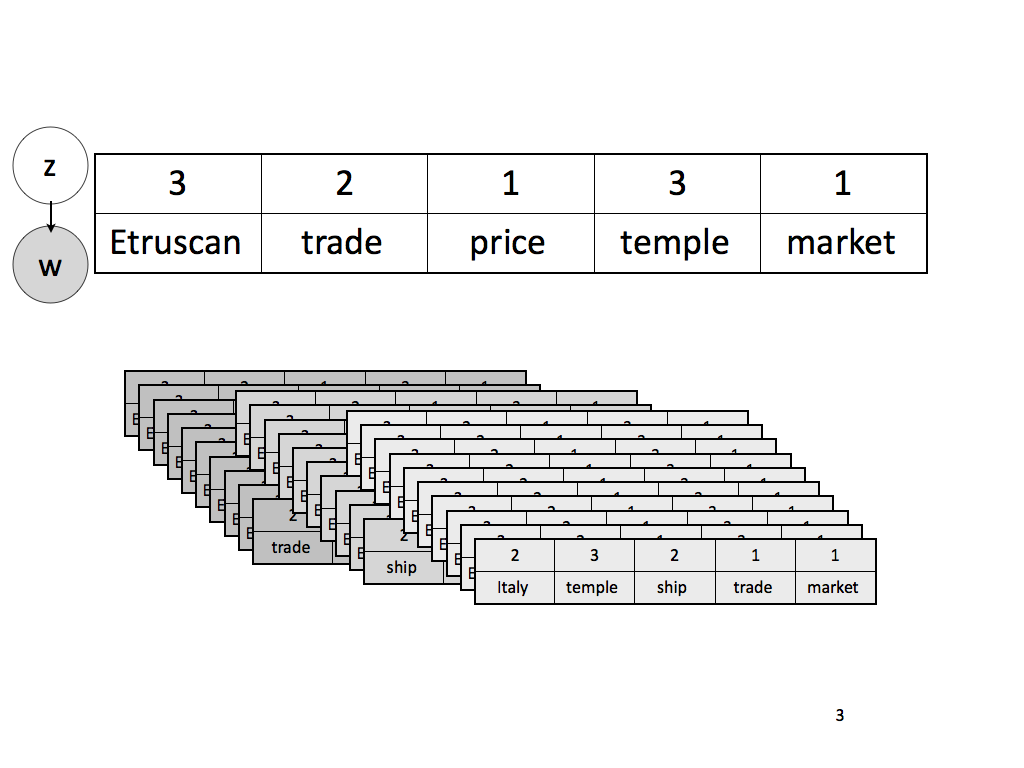
\includegraphics[width=\linewidth]{topic_models/mimno_003}
\end{frame}

\begin{frame}
  \frametitle{Total Topic Counts}
    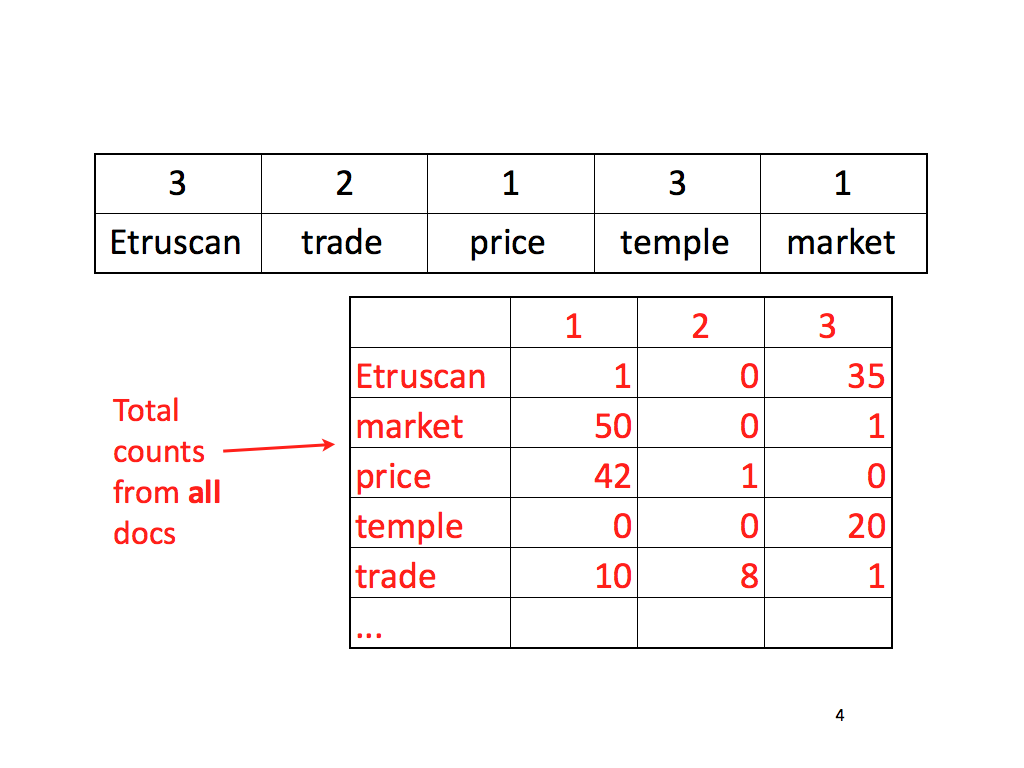
\includegraphics[width=\linewidth]{topic_models/mimno_004}

\pause

\vspace{-3cm}

\begin{block}{Sampling Equation}
	\begin{equation*}
          \frac{n_{d, k} + \alpha_k}{ \sum_{i}^{K} { n_{d,i} + \alpha_i}} \frac{\alert<3>{v_{k, w_{d,n}}} + \lambda_{w_{d,n}}}{ \sum_{i} { \alert<3>{v_{k,i}} + \lambda_{i} }}
	\end{equation*}
\end{block}

\end{frame}


\begin{frame}
  \frametitle{We want to sample this word \dots}
    \only<1>{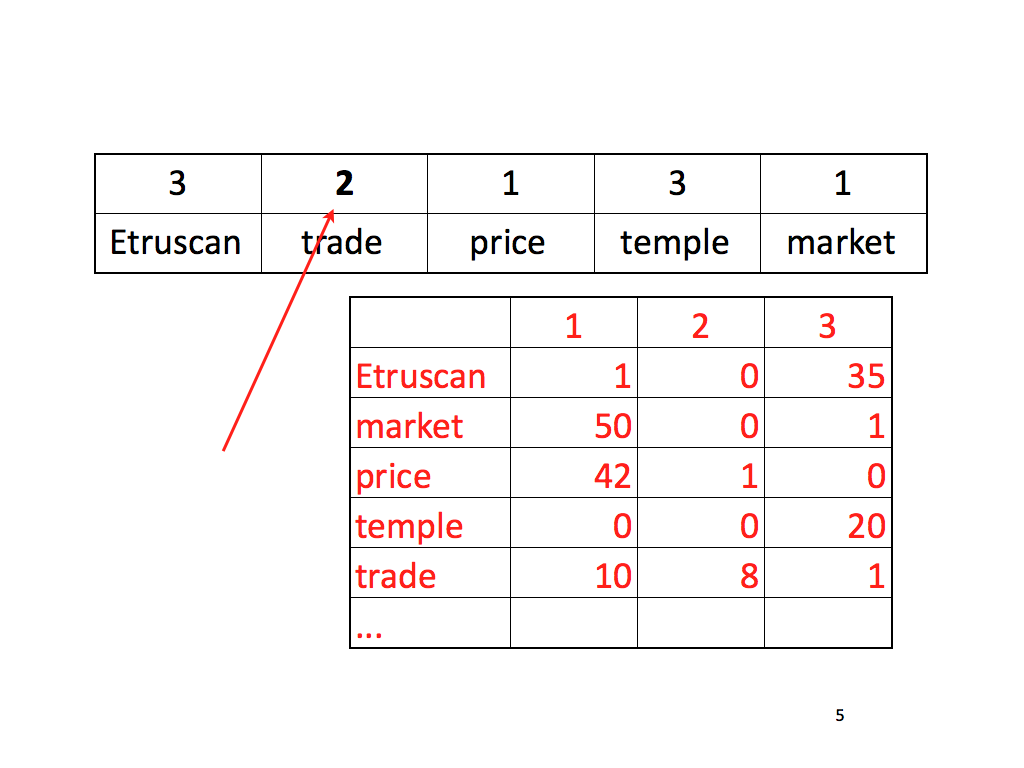
\includegraphics[width=\linewidth]{topic_models/mimno_005}}
    \only<2>{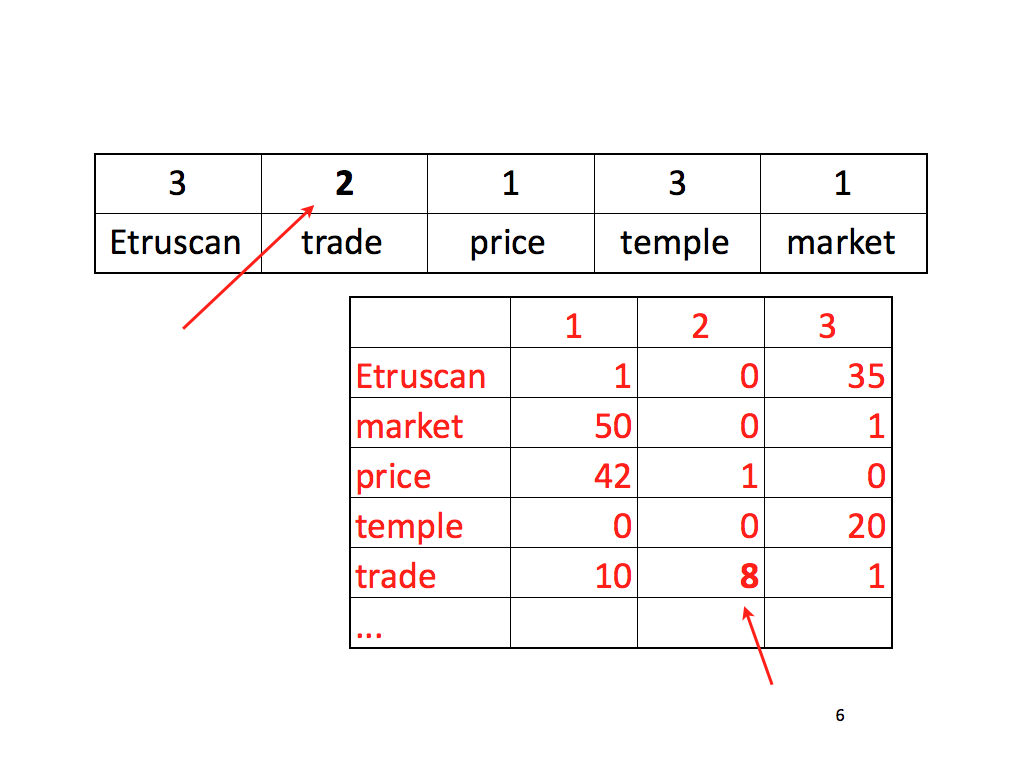
\includegraphics[width=\linewidth]{topic_models/mimno_006}}
\end{frame}

\begin{frame}
  \frametitle{Decrement its count}
    \includegraphics[width=\linewidth]{topic_models/mimno_007}
\end{frame}

\begin{frame}
  \frametitle{What is the conditional distribution for this topic?}
    \includegraphics[width=\linewidth]{topic_models/mimno_008}
\end{frame}


\begin{frame}
  \frametitle{Part 1: How much does this document like each topic?}
    \includegraphics[width=\linewidth]{topic_models/mimno_008}
\end{frame}

\begin{frame}
  \frametitle{Part 1: How much does this document like each topic?}
    \includegraphics[width=\linewidth]{topic_models/mimno_009}

    \pause
    \vspace{-4cm}
    \begin{block}{Sampling Equation}
	\begin{equation*}
          \frac{\alert<3>{n_{d, k}} + \alpha_k}{ \sum_{i}^{K} { \alert<3>{n_{d,i}} + \alpha_i}} \frac{v_{k, w_{d,n}} + \lambda_{w_{d,n}}}{ \sum_{i} { v_{k,i} + \lambda_{i} }}
	\end{equation*}
     \end{block}


\end{frame}


\begin{frame}
  \frametitle{Part 2: How much does each topic like the word?}
    \includegraphics[width=\linewidth]{topic_models/mimno_010}

\pause

\vspace{-3cm}

\begin{block}{Sampling Equation}
	\begin{equation*}
          \frac{n_{d, k} + \alpha_k}{ \sum_{i}^{K} { n_{d,i} + \alpha_i}} \frac{\alert<3>{v_{k, w_{d,n}}} + \lambda_{w_{d,n}}}{ \sum_{i} { \alert<3>{v_{k,i}} + \lambda_{i} }}
	\end{equation*}
\end{block}

\end{frame}


\begin{frame}
  \frametitle{Geometric interpretation}
    \only<1>{\includegraphics[width=\linewidth]{topic_models/mimno_011}}
    \only<2>{\includegraphics[width=\linewidth]{topic_models/mimno_012}}
    \only<3>{\includegraphics[width=\linewidth]{topic_models/mimno_013}}
\end{frame}

\begin{frame}
  \frametitle{Update counts}
    \only<1>{\includegraphics[width=\linewidth]{topic_models/mimno_014}}
    \only<2>{\includegraphics[width=\linewidth]{topic_models/mimno_015}}
    \only<3>{\includegraphics[width=\linewidth]{topic_models/mimno_016}}
\end{frame}


\begin{frame}
  \frametitle{Details: how to sample from a distribution}

\begin{center}
  \includegraphics[width=.8\linewidth]{topic_models/sampling_from_distribution}
\end{center}
\end{frame}

\begin{frame}

\begin{block}{Algorithm}
\begin{enumerate}
\item For each iteration $i$:
\begin{enumerate}
\item For each document $d$ and word $n$ currently assigned to $z_{old}$:
\begin{enumerate}
\item Decrement $n_{d,z_{old}}$ and $v_{z_{old}, w_{d,n}}$
\item Sample $z_{new} = k$ with probability proportional to $\frac{n_{d, k} + \alpha_k}{ \sum_{i}^{K} { n_{d,i} + \alpha_i}} \frac{v_{k, w_{d,n}} + \lambda_{w_{d,n}}}{ \sum_{i} { v_{k,i} + \lambda_{i}}}$
\item Increment $n_{d,z_{new}}$ and $v_{z_{new}, w_{d,n}}$
\end{enumerate}
\end{enumerate}
\end{enumerate}
\end{block}

\end{frame}

\begin{frame}

\frametitle{Implementation}

\begin{block}{Algorithm}
\begin{enumerate}
\item For each iteration $i$:
\begin{enumerate}
\item For each document $d$ and word $n$ currently assigned to $z_{old}$:
\begin{enumerate}
\item Decrement $n_{d,z_{old}}$ and $v_{z_{old}, w_{d,n}}$
\item Sample $z_{new} = k$ with probability proportional to $\frac{n_{d, k} + \alpha_k}{ \sum_{i}^{K} { n_{d,i} + \alpha_i}} \frac{v_{k, w_{d,n}} + \lambda_{w_{d,n}}}{ \sum_{i} { v_{k,i} + \lambda_{i}}}$
\item Increment $n_{d,z_{new}}$ and $v_{z_{new}, w_{d,n}}$
\end{enumerate}
\end{enumerate}
\end{enumerate}
\end{block}

\end{frame}


\begin{frame}
\frametitle{Desiderata}
\begin{itemize}
\item Hyperparameters: Sample them too (slice sampling)
\item Initialization: Random
\item Sampling: Until likelihood converges
\item Lag / burn-in: Difference of opinion on this
\item Number of chains: Should do more than one
\end{itemize}
\end{frame}

\begin{frame}
	\frametitle{Available implementations}

	\begin{itemize}
		\item Mallet (http://mallet.cs.umass.edu)
		\item LDAC (http://www.cs.princeton.edu/~blei/lda-c)
		\item Topicmod (http://code.google.com/p/topicmod)
	\end{itemize}
\end{frame}

\section{Mallet Tutorial}



\begin{frame}{Mallet}

\begin{itemize}
  \item Developed at UMass Amherst by Andrew McCallum and David Mimno (among others)
  \item Very fast implementation of Gibbs sampling for topic modeling
  \item (Somewhat) friendly interface
  \item Easiest on \textsc{unix}-derived operating systems, but also works on Windows
  \item Requires Java
\end{itemize}

\begin{columns}
\column{.5\linewidth}
\begin{block}{Download Location}
  http://mallet.cs.umass.edu/
\end{block}
\column{.5\linewidth}
\includegraphics[width=.9\linewidth]{topic_models/mallet}
\end{columns}
\end{frame}


\begin{frame}
  \frametitle{Scenario}

  \begin{itemize}
    \item Learn a (small-sized) topic model on \textsc{nsf} data
    \item Apply those topics to \textsc{nrc} data
    \item Discover the priorities of \textsc{nsf}
    \item Connects \textsc{nrc} grants to that model
    \item Walk through the commands to do everything
  \end{itemize}
\end{frame}

\begin{frame}[fragile]


\frametitle {Getting Your Data}

\begin{columns}
  \column{.6\linewidth}
    \begin{itemize}
      \item Text file separated by columns
      \item \alert<1>{First column: doc id}
      \item \alert<2>{Second column: language}
      \item \alert<3>{Third column: text}
    \end{itemize}
  \column{.3\linewidth}
     \begin{tabular}{lll}
       \alert<1>{doc} & \alert<2>{lang} & \alert<3>{text} \\
     \end{tabular}
\end{columns}

\begin{block}{Download}
  \url{http://umiacs.umd.edu/~jbg/lda_demo/nsf-30k.txt}
\end{block}

\pause \pause \pause \pause 
\begin{lstlisting}
doc0    none    It is proposed to grow and characterize ternary alloys of ...
doc1    none    This project will focus on development of new cutting tool designs ...
doc2    none    The purpose of the proposed work is to design a novel cooling device ...
doc3    none    The objective of this research project is to develop a wireless ...
\end{lstlisting}

\end{frame}


\begin{frame}[fragile]

  \frametitle{Preparing \textsc{nsf} Data}

  \begin{block}{Mallet Command}
    mallet \alert<2>{import-file} \alert<3>{--remove-stopwords} \alert<4>{--keep-sequence} \alert<5>{--input ~/data/nsf\_abstracts/nsf-30k.txt} \alert<6>{--output nsf.mallet}
  \end{block}

  \pause

  \begin{itemize}
    \item \alert<2>{Tell Mallet what to do}
    \item \alert<3>{Remove words like ``the'', ``and'', ``of''} (otherwise, they'd be at the top of every topic)
    \item \alert<4>{Remember the order of words} (required for Gibbs sampling)
    \item \alert<5>{The input text file}
    \item \alert<6>{Where it writes the binary file}
  \end{itemize}

\end{frame}

\begin{frame}
  \frametitle{Preparing \textsc{nrc} data}

  \begin{block}{Mallet Command}
    mallet import-file --remove-stopwords --keep-sequence --input ~/data/norwegian\_research/merged.txt --output nrc.mallet \alert<2>{--use-pipe-from nsf.mallet}
  \end{block}

  \begin{itemize}
    \item Nearly identical to previous command
    \pause
    \item Main difference: use \textsc{nsf} vocabulary to encode the data
    \item \textsc{lda} doesn't know what words mean
    \item Internally, these algorithms map words to numbers: oxygen (2134), neutrino (33), Weber (1701)
    \item This ensures that this mapping is consistent between datasets
   \end{itemize}

\end{frame}


\begin{frame}
  \frametitle{Fitting a topic model}

\begin{block}{Mallet Command}
\small
  mallet train-topics --input \alert<2>{nsf.mallet}  --num-topics \alert<3>{10} --num-iterations \alert<4>{100} --output-model \alert<5>{nsf\_10.model} --output-state \alert<6>{nsf\_10.state.gz} --output-doc-topics \alert<7>{nsf\_10.doc} --output-topic-keys \alert<8>{nsf\_10.topics} --inferencer-filename \alert<9>{nsf\_10.inf}
\end{block}

\pause

\begin{columns}

  \column{.65\linewidth}

  \begin{itemize}
    \item The \alert<2>{documents} we learn topics from 
    \item The \alert<3>{number of topics} we'll learn
    \item The \alert<4>{number of sweeps} through data
    \item Save the \alert<5>{resulting model}
    \item Save \alert<6>{Gibbs sampling states}
    \item Save \alert<7>{document-topic associations}
    \item Save \alert<8>{word-topic associations}
    \item Save \alert<9>{inferencer}
  \end{itemize}

  \column{.3\linewidth}
    \only<2>{\includegraphics[width=0.9\linewidth]{topic_models/newspapers} }
    \only<6>{\includegraphics[width=.6\linewidth]{topic_models/inference_3}}
    \only<7>{\includegraphics[width=0.9\linewidth]{topic_models/nyt_documents}}
    \only<8>{\includegraphics[width=0.9\linewidth]{reading_tea_leaves/figures/nyt_topics_wide}}  
    \only<9>{
    \begin{block}{Inferencer}
        Allows us to apply these topics to another dataset
      \end{block}
    }
  \end{columns}

\end{frame}

\begin{frame}[fragile]
  \frametitle{As Mallet Runs \dots}

  \begin{lstlisting}
<10> LL/token: -10,01271
<20> LL/token: -9,17157
<30> LL/token: -9,01933
<40> LL/token: -8,96692
  \end{lstlisting}

  \begin{itemize}
    \item we want to discover best collection of topics that describes our data
      \item this is defined in terms of probability
        \item stochastic search
          \begin{itemize}
            \item stop when probability levels off
              \item requires thousands of iterations
            \end{itemize}
    \end{itemize}

\end{frame}

\begin{frame}[fragile]
  \frametitle{As Mallet Runs \dots}

  \begin{lstlisting}
0	5	species environmental water natural understanding study research processes climate change ocean global carbon studies production marine important conditions populations effects 
1	5	materials research chemistry properties chemical high magnetic optical surface electron state phase structures structure devices electronic metal molecular studies program 
2	5	systems system design research data control performance network based time applications develop software techniques proposed power application networks developed high 
  \end{lstlisting}

  \begin{itemize}
    \item ID of the topic
    \item Weight of the topic (start the same)
    \item The most probable words in the topic
   \end{itemize}

\end{frame}

\begin{frame}[fragile]
  \frametitle{Word-Topic Association}
  \begin{lstlisting}
0       5       species environmental water natural understanding study research processes climate change ocean global carbon production studies marine populations conditions important long 
1       5       materials research chemistry properties chemical high magnetic optical surface electron phase state structures structure molecular devices electronic metal studies program 
    \end{lstlisting}

    \begin{itemize}
      \item Same information as displayed as Mallet runs
        \item Shows the most probable words in each topic
      \end{itemize}

\end{frame}


\begin{frame}{What topics did we discover?}
\small
  \begin{enumerate}
    \setcounter{enumi}{-1}
    \item {\bf Environmental Science}: climate ocean environmental marine species
    \item {\bf Materials Science}: materials chemistry properties magnetic structure
    \item {\bf Systems Engineering}: control network applications power software
    \item {\bf Social Science}: economic social human policy behavior public
    \item {\bf Training}: undergraduate education program students graduate training
    \item {\bf Physics}: mass energy time flow scale mass rate phase energy
    \item {\bf biology}: cell protein molecular function genes proteins gene cells
    \item {\bf Computer Science}: information web computer research industry
    \item {\bf Geology}: region earth ice provide field sites events mantle deep seismic 
    \item {\bf Math}: theory methods problem mathematical analysis number geometry
    \end{enumerate}
\end{frame}

\begin{frame}[fragile]
  \frametitle{What documents are associated with each topic?}

  \begin{lstlisting}
138     doc138  8       0.291970802919708       4       0.24087591240875914     0
       0.08759124087591241     3       0.072992700729927       7       0.06569343065693431     9       0.051094890510948905    5       0.051094890510948905    1       0.051094890510948905    6       0.043795620437956206    2       0.043795620437956206
139     doc139  4       0.304   5       0.168   6       0.104   9       0.08    8
       0.072   7       0.064   0       0.064   3       0.048   2       0.048   1
       0.048  
    \end{lstlisting}

    \begin{itemize}
      \item Document 138 is associated with topic 4 and topic 8
        \item These are the Training and Geology topics
      \end{itemize}

      \pause

      \vspace{-3cm}

  \begin{block}{doc138}
    \small
This Americas Program award will support a planning visit 
dots  to carry out join research planning with scientists of the Instituto, to investigate field logistics, and examining key field sites, with the goal of developing two joint research projects, as well as a joint training program for advanced students of active tectonics and geologic hazards. The projects include a study of the geodynamic mass balance in the northern Andes between volcanic eruptions and erosion; study of neotectonic deformation and catastrophic sedimentation in the Interandean Valley
  \end{block}

\end{frame}


\begin{frame}
  \frametitle{Applying topics to \textsc{nrc} data}
  \begin{itemize}
    \item Assume that we are satisfied with this topic analysis
    \item \textsc{nsf} is convenient example
      \begin{itemize}
        \item \textsc{eu}-wide research
        \item Wikipedia
        \item Publications
      \end{itemize}
      \item Associate \alert<2>{new documents} with some \alert<3>{standard}
      \item Compare funding levels for comparable topics (regardless of internal classification)
  \end{itemize}

\end{frame}


\begin{frame}
  \frametitle{Applying Topics}
    \begin{block}{Mallet Command}
      mallet infer-topics --input \alert<2>{nrc.mallet} --inferencer \alert<3>{nsf\_10.inf} --output-doc-topics \alert<4>{nrc.doc}
    \end{block}

    \begin{itemize}
      \item Document to apply model to
      \item Inferencer created from model
      \item Output file
    \end{itemize}

\end{frame}

\begin{frame}
  \frametitle{Much more to be done!}

  \begin{itemize}
    \item Bigrams: not all strings separated by spaces are words
      \begin{itemize}
        \item high energy, nano materials, seismic models, undergraduate students
          \item need to be discovered along with topics
        \end{itemize}
        \item Choosing correct granularity
        \item Refining stopword list: investigator, study, research
        \item \alert<2>{Adding constraints}
        \item \alert<2>{Multiple languages}
   \end{itemize}

\end{frame}

\section{Research / Extensions}


\frame{

\frametitle{The Problem: User Perspective}

\begin{columns}

\column{.4\linewidth}
\begin{center}
\begin{tabular}{ccc}
& \only<2->{\itmspace}\color<2->{red}{bladder} & \\
& \only<3->{\hspace{-2cm}} \color<3->{blue}{spinal\_cord}  & \\
& \only<3->{\hspace{-2cm}} \color<3->{blue}{sci} & \\
& \only<3->{\hspace{-2cm}}\color<3->{blue}{spinal\_cord\_injury} & \\
& \only<3->{\hspace{-2cm}}\color<3->{blue}{spinal} & \\
& \only<2->{\itmspace}\color<2->{red}{urinary} & \\
& \only<2->{\itmspace}\color<2->{red}{urothelial} & \\
& \only<3->{\hspace{-2cm}}\color<3->{blue}{cervical} & \\
& injury & \\
& recovery & \\
& \only<2->{\itmspace}\color<2->{red}{urinary\_tract} & \\
& locomotor & \\
& \only<3->{\hspace{-2cm}}\color<3->{blue}{lumbar} & \\
\end{tabular}
\end{center}

\column{.6\linewidth}

\danquote{These words don't belong together!}

\end{columns}

}

\begin{frame}
        \frametitle{This is serious business!}


        \begin{itemize}
          \item Decision makers see problems
          \item No easy way to correct the problem
          \item Result: entire approach is abandoned
\pause
          \item Offer support for two kinds of feedback~\cite{boyd-graber-07,andrzejewski-09}
            \begin{itemize}
              \item Positive correlations: words that {\bf should} appear together
              \item Negative correlations: words that {\bf should not} appear together
            \end{itemize}
        \end{itemize}

\end{frame}




\frame{
	\frametitle{How to incorporate feedback?}

	\begin{columns}

	\column{.5\linewidth}

		\begin{columns}

			\column{.6\linewidth}

			\includegraphics[width=\linewidth]{topic_models/nyt_topics}


			\column{.4\linewidth}
			\begin{center}
				\only<2->{\includegraphics[width=.6\linewidth]{general_figures/arrow_right_down} \\}
				\only<2->{\includegraphics[width=.6\linewidth]{general_figures/milkman_dan} \\}
				\invisible<-2>{\includegraphics[width=.6\linewidth,angle=270]{general_figures/arrow_right_down}}
			\end{center}

		\end{columns}

	\column{.5\linewidth}

	\begin{enumerate}
		\item Fit initial topic model
			\pause
		\item Get feedback from user
			\pause
		\item Incrementally relearn model
			\begin{itemize}
                                \item Forget your mistakes
				\item Replace the model with a correlated one
				\item Continue inference
			\end{itemize}
	\end{enumerate}
\pause
Keep computation \alert<4>{fast and consistent} \cite{Hu-12a}
	\end{columns}

}

\providecommand{\tb}[1]{\parbox{0.8\linewidth}{ \tiny{ #1 }} \vspace{.2cm} }

\frame{

\vspace{-1cm}

\begin{columns}

\column{.5\linewidth}

\begin{tabular}{l*{2}{c}r}
	Topic & Before \\
\hline

\alert<2>{{\bf 1}} & \tb{ \alert<2>{election, yeltsin, russian, political, party, democratic, russia,
  president, democracy, boris, country, south, years, month, government, vote,
  since, leader, presidential, military} } \\

2 & \tb{new, york, city, state, mayor, budget, giuliani, council, cuomo, gov,
  plan, year, rudolph, dinkins, lead, need, governor, legislature, pataki,
  david} \\

3 & \tb{nuclear, arms, weapon, defense, treaty, missile, world, unite, yet,
  soviet, lead, secretary, would, control, korea, intelligence, test, nation,
  country, testing} \\

4 & \tb{president, bush, administration, clinton, american, force, reagan, war,
  unite, lead, economic, iraq, congress, america, iraqi, policy, aid,
  international, military, see} \\

& \vdots \\

\alert<2>{{\bf 20}} & \tb{\alert<2>{soviet, lead, gorbachev, union, west, mikhail, reform, change, europe,
  leaders, poland, communist, know, old, right, human, washington, western,
  bring, party} }\\

\end{tabular}

\column{.5\linewidth}

\only<3> {

	\begin{block}{Suggestion}
	\emph{boris, communist, gorbachev, mikhail, russia,
  russian, soviet, union, yeltsin }
	\end{block}

}

\only<4-> {

\begin{tabular}{l*{2}{c}r}
	Topic & After \\
\hline

\alert<5>{{\bf 1}} & \alert<5>{\tb{election, democratic, south, country, president, party, africa, lead,
  even, democracy, leader, presidential, week, politics, minister, percent,
  voter, last, month, years} } \\

\alert<6>{2} & \tb{new, york, city, state, mayor, budget, council, giuliani, gov, cuomo,
  year, rudolph, dinkins, legislature, plan, david, governor, pataki, need, cut}
\\

\alert<6>{3} & \tb{nuclear, arms, weapon, treaty, defense, war, missile, may, come, test,
  american, world, would, need, lead, get, join, yet, clinton, nation} \\

\alert<6>{4} & \tb{president, administration, bush, clinton, war, unite, force, reagan,
  american, america, make, nation, military, iraq, iraqi, troops, international,
  country, yesterday, plan} \\

   & \vdots \\

\alert<4>{ {\bf 20} } & \alert<4> {\tb{soviet, union, economic, reform, yeltsin, russian, lead, russia,
  gorbachev, leaders, west, president, boris, moscow, europe, poland, mikhail,
  communist, power, relations} } \\

\end{tabular}

}

\end{columns}

}


\providecommand{\blue}[1]{{\color{blue}{#1}}}
\providecommand{\red}[1]{{\color{red}{#1}}}
\providecommand{\green}[1]{{\color{green}{#1}}}

\begin{frame}

\frametitle{Example: Negative Constraint}

\begin{columns}

\column{.4\linewidth}

\begin{tabular}{l*{2}{c}r}
	Topic & Words \\
\hline

{\bf 318} & \tb{\red{bladder}, sci, \blue{spinal\_cord}, \blue{spinal\_cord\_injury}, \blue{spinal}, \red{urinary}, \red{urinary\_tract}, \red{urothelial},\blue{injury}, \blue{motor}, \blue{recovery}, \blue{reflex}, \blue{cervical}, \red{urothelium}, \blue{functional\_recovery}} \\

\end{tabular}

\column{.1\linewidth}

\column{.4\linewidth}

\only<3->{
\begin{tabular}{l*{2}{c}r}
	Topic & Words \\
\hline

{\bf 318} & \tb{sci, \blue{spinal\_cord}, \blue{spinal\_cord\_injury}, \blue{spinal}, \blue{injury}, \blue{recovery}, \blue{motor}, \blue{reflex}, \red{urothelial}, \green{injured}, \blue{functional\_recovery}, \green{plasticity}, \green{locomotor}, \blue{cervical}, \green{locomotion}}\\

\end{tabular}
}

\end{columns}

\only<2->{
\begin{block}{Negative Constraint}
  spinal\_cord, bladder
\end{block}

}

\end{frame}




\frame{
\frametitle{Evaluation}
\begin{center}
%\only<1>{\includegraphics[width=0.9\linewidth]{reading_tea_leaves/figures/heldout_1} }
\only<1>{\includegraphics[width=\linewidth]{reading_tea_leaves/figures/heldout_2} }
%\only<3>{\includegraphics[width=\linewidth]{reading_tea_leaves/figures/heldout_3} }
\only<2>{\includegraphics[width=\linewidth]{reading_tea_leaves/figures/heldout_4}  \\
	\large Measures predictive power, not what the topics are}
\end{center}

\begin{center}
\includegraphics[width=0.5\linewidth]{topic_models/equations/evaluation} \\
How you compute it is important too~\cite{wallach-09b}
\end{center}

}

\frame{
  \frametitle{Word Intrusion}

  \includegraphics[width=\linewidth]{reading_tea_leaves/figures/nyt_topics_wide}
}


\frame{
  \frametitle{Word Intrusion}

  \begin{enumerate}
    \item Take the highest probability words from a topic

      \begin{block}{Original Topic}
        dog, cat, horse, pig, cow
      \end{block}
\pause
    \item Take a high-probability word from another topic and add it
      \begin{block}{Topic with Intruder}
        dog, cat, \alert<2->{apple}, horse, pig, cow
      \end{block}
\pause
     \item We ask users to find the word that doesn't belong
  \end{enumerate}
\begin{block}{Hypothesis}
If the topics are interpretable, users will consistently choose true intruder
\end{block}
}

\frame{
\frametitle{Word Intrusion}
\begin{center}
\only<1>{\includegraphics[width=\linewidth]{reading_tea_leaves/tasks/word1}  }
\only<2>{\includegraphics[width=\linewidth]{reading_tea_leaves/tasks/word2}  }
\pause
  \begin{itemize}
    \item Order of words was shuffled
    \item Which intruder was selected varied
    \item Model precision: percentage of users who clicked on intruder
  \end{itemize}

\end{center}
}

\frame{
\frametitle{Word Intrusion: Which Topics are Interpretable?}
  \begin{block}{New York Times, 50 LDA Topics}
    \begin{center}
      \includegraphics[width=0.8\linewidth]{reading_tea_leaves/figures/topic_precision}
    \end{center}
  \end{block}
  \begin{center}
    Model Precision: percentage of correct intruders found
  \end{center}
}



\frame{

\frametitle{Interpretability and Likelihood}
\begin{center}
\only<1>{Model Precision on New York Times}
\only<2>{Topic Log Odds on Wikipedia}
\end{center}

\begin{columns}
\column{.85\linewidth}
\begin{flushright}
  \only<1>{\includegraphics[scale=\graphscale]{reading_tea_leaves/tasks/mp}}
  \only<2>{\includegraphics[scale=\graphscale]{reading_tea_leaves/tasks/tlo}}
  \only<1>{\includegraphics[scale=\graphscale]{reading_tea_leaves/tasks/mp_y}\includegraphics[scale=\graphscale]{reading_tea_leaves/tasks/nyt_mp}}
  \only<2>{\includegraphics[scale=\graphscale]{reading_tea_leaves/tasks/tlo_y}\includegraphics[scale=\graphscale]{reading_tea_leaves/tasks/wiki_tlo}} \\
  \only<1>{\includegraphics[scale=\graphscale]{reading_tea_leaves/tasks/nyt_x}}
  \only<2>{\includegraphics[scale=\graphscale]{reading_tea_leaves/tasks/wiki_x}}
\end{flushright}
\column{.15\linewidth}
  \includegraphics[scale=\graphscale]{reading_tea_leaves/tasks/legend}
\end{columns}
\vspace{-0.75cm}
\begin{center}
  \includegraphics[scale=\graphscale]{reading_tea_leaves/tasks/held-out} \\
\only<1> {within a model, higher likelihood $\not =$ higher interpretability}
\only<2> {across models, higher likelihood $\not =$ higher interpretability}
\end{center}
}


\begin{frame}
  \frametitle{Evaluation Takeaway}

  \begin{itemize}
    \item Measure what you care about~\cite{chang-09c}
      \item If you care about prediction, likelihood is good
\item If you care about a particular task, measure that
    \end{itemize}

\end{frame}


\begin{frame}{Other Research: Hierarchical Models}
   \begin{center}
   \only<1>{ \includegraphics[width=0.8\linewidth]{shlda/ideology_topics}}
   \only<2>{ \includegraphics[width=1.0\linewidth]{shlda/amazon_topics}}
   \only<3>{ \includegraphics[width=0.7\linewidth]{shlda/amazon_topics_zoom}}
   \end{center}
\end{frame}

\begin{frame}{Other Research: Incorporating New Words}
  \only<1>{\includegraphics[width=\linewidth]{infvoc/new_words_highlight_1}}
  \only<2>{\includegraphics[width=\linewidth]{infvoc/new_words_highlight_2}}
  \only<3>{\includegraphics[width=\linewidth]{infvoc/new_words_highlight_3}}
  \only<4>{\includegraphics[width=\linewidth]{infvoc/new_words_highlight_4}}
  \only<5>{\includegraphics[width=\linewidth]{infvoc/new_words_highlight_5}}
  \only<6>{\includegraphics[width=\linewidth]{infvoc/new_words_highlight_6}}
  \only<7>{\includegraphics[width=\linewidth]{infvoc/new_words_highlight_7}}
  \only<8>{\includegraphics[width=\linewidth]{infvoc/new_words_highlight_8}}
%\end{figure}
%\end{center}
\begin{center}
\vspace{-5mm}
An example topic from \textit{20 newsgroups} under our model.
Numbers preceeding words are ranks in topic.
\end{center}

\end{frame}


\section{Conclusion}

\begin{frame}{Topic Models for Large Text Collections}

  \begin{itemize}
    \item Unsupervised tool for understanding large text collections
    \item Statistical foundation
    \item Open source tools for learning these models
    \item Example application to \textsc{nsf} and \textsc{nrc} data
  \end{itemize}

\end{frame}

\frame{

	\frametitle{Thanks}

        \begin{block}{Collaborators}
          Yuening Hu (UMD), Ke Zhai (UMD), Viet-An Nguyen (UMD), Dave Blei
          (Princeton), Jonathan Chang (Facebook), Philip Resnik (UMD), Christiane Fellbaum (Princeton), Jerry
          Zhu (Wisconsin), Sean Gerrish (Sift), Chong Wang (CMU), Dan Osherson
          (Princeton), Sinead Williamson (CMU)
        \end{block}

        \begin{block}{Funders}
        \end{block}
        \begin{center}
          \includegraphics[width=0.2\linewidth]{general_figures/nsf}
          \hspace{0.5cm}
          \includegraphics[width=0.2\linewidth]{general_figures/arl}
          \hspace{0.5cm}
          \includegraphics[width=0.2\linewidth]{general_figures/iarpa}
          \hspace{0.5cm}
          \includegraphics[width=0.2\linewidth]{general_figures/lockheed-martin}
       \end{center}

}


\begin{frame}
\bibliographystyle{plain}
\tiny
\bibliography{bib/journal-full,bib/jbg}
\end{frame}

\end{document}
